\documentclass[twoside]{book}

% Packages required by doxygen
\usepackage{calc}
\usepackage{doxygen}
\usepackage{graphicx}
\usepackage[utf8]{inputenc}
\usepackage{makeidx}
\usepackage{multicol}
\usepackage{multirow}
\usepackage{textcomp}
\usepackage[table]{xcolor}

% Font selection
\usepackage[T1]{fontenc}
\usepackage{mathptmx}
\usepackage[scaled=.90]{helvet}
\usepackage{courier}
\usepackage{amssymb}
\usepackage{sectsty}
\renewcommand{\familydefault}{\sfdefault}
\allsectionsfont{%
  \fontseries{bc}\selectfont%
  \color{darkgray}%
}
\renewcommand{\DoxyLabelFont}{%
  \fontseries{bc}\selectfont%
  \color{darkgray}%
}

% Page & text layout
\usepackage{geometry}
\geometry{%
  a4paper,%
  top=2.5cm,%
  bottom=2.5cm,%
  left=2.5cm,%
  right=2.5cm%
}
\tolerance=750
\hfuzz=15pt
\hbadness=750
\setlength{\emergencystretch}{15pt}
\setlength{\parindent}{0cm}
\setlength{\parskip}{0.2cm}
\makeatletter
\renewcommand{\paragraph}{%
  \@startsection{paragraph}{4}{0ex}{-1.0ex}{1.0ex}{%
    \normalfont\normalsize\bfseries\SS@parafont%
  }%
}
\renewcommand{\subparagraph}{%
  \@startsection{subparagraph}{5}{0ex}{-1.0ex}{1.0ex}{%
    \normalfont\normalsize\bfseries\SS@subparafont%
  }%
}
\makeatother

% Headers & footers
\usepackage{fancyhdr}
\pagestyle{fancyplain}
\fancyhead[LE]{\fancyplain{}{\bfseries\thepage}}
\fancyhead[CE]{\fancyplain{}{}}
\fancyhead[RE]{\fancyplain{}{\bfseries\leftmark}}
\fancyhead[LO]{\fancyplain{}{\bfseries\rightmark}}
\fancyhead[CO]{\fancyplain{}{}}
\fancyhead[RO]{\fancyplain{}{\bfseries\thepage}}
\fancyfoot[LE]{\fancyplain{}{}}
\fancyfoot[CE]{\fancyplain{}{}}
\fancyfoot[RE]{\fancyplain{}{\bfseries\scriptsize Generated on Wed Dec 4 2013 05\-:53\-:54 for Pirate Adventures by Doxygen }}
\fancyfoot[LO]{\fancyplain{}{\bfseries\scriptsize Generated on Wed Dec 4 2013 05\-:53\-:54 for Pirate Adventures by Doxygen }}
\fancyfoot[CO]{\fancyplain{}{}}
\fancyfoot[RO]{\fancyplain{}{}}
\renewcommand{\footrulewidth}{0.4pt}
\renewcommand{\chaptermark}[1]{%
  \markboth{#1}{}%
}
\renewcommand{\sectionmark}[1]{%
  \markright{\thesection\ #1}%
}

% Indices & bibliography
\usepackage{natbib}
\usepackage[titles]{tocloft}
\setcounter{tocdepth}{3}
\setcounter{secnumdepth}{5}
\makeindex

% Hyperlinks (required, but should be loaded last)
\usepackage{ifpdf}
\ifpdf
  \usepackage[pdftex,pagebackref=true]{hyperref}
\else
  \usepackage[ps2pdf,pagebackref=true]{hyperref}
\fi
\hypersetup{%
  colorlinks=true,%
  linkcolor=blue,%
  citecolor=blue,%
  unicode%
}

% Custom commands
\newcommand{\clearemptydoublepage}{%
  \newpage{\pagestyle{empty}\cleardoublepage}%
}


%===== C O N T E N T S =====

\begin{document}

% Titlepage & ToC
\hypersetup{pageanchor=false}
\pagenumbering{roman}
\begin{titlepage}
\vspace*{7cm}
\begin{center}%
{\Large Pirate Adventures }\\
\vspace*{1cm}
{\large Generated by Doxygen 1.8.5}\\
\vspace*{0.5cm}
{\small Wed Dec 4 2013 05:53:54}\\
\end{center}
\end{titlepage}
\clearemptydoublepage
\tableofcontents
\clearemptydoublepage
\pagenumbering{arabic}
\hypersetup{pageanchor=true}

%--- Begin generated contents ---
\chapter{Hierarchical Index}
\section{Class Hierarchy}
This inheritance list is sorted roughly, but not completely, alphabetically\-:\begin{DoxyCompactList}
\item \contentsline{section}{anim\-Items}{\pageref{classanim_items}}{}
\item \contentsline{section}{attack\-List}{\pageref{classattack_list}}{}
\item \contentsline{section}{attackmove}{\pageref{classattackmove}}{}
\begin{DoxyCompactList}
\item \contentsline{section}{brokengun}{\pageref{classbrokengun}}{}
\item \contentsline{section}{brokenshot}{\pageref{classbrokenshot}}{}
\item \contentsline{section}{Hookslash}{\pageref{class_hookslash}}{}
\item \contentsline{section}{shotgun}{\pageref{classshotgun}}{}
\item \contentsline{section}{swordslash}{\pageref{classswordslash}}{}
\item \contentsline{section}{xgun}{\pageref{classxgun}}{}
\end{DoxyCompactList}
\item \contentsline{section}{Character}{\pageref{class_character}}{}
\item Q\-Dialog\begin{DoxyCompactList}
\item \contentsline{section}{attackframe}{\pageref{classattackframe}}{}
\item \contentsline{section}{Battle\-Pause}{\pageref{class_battle_pause}}{}
\item \contentsline{section}{Pause}{\pageref{class_pause}}{}
\item \contentsline{section}{worldmap}{\pageref{classworldmap}}{}
\end{DoxyCompactList}
\item Q\-Graphics\-Item\begin{DoxyCompactList}
\item \contentsline{section}{Map\-Enemy}{\pageref{class_map_enemy}}{}
\item \contentsline{section}{Map\-Hero}{\pageref{class_map_hero}}{}
\end{DoxyCompactList}
\item Q\-Main\-Window\begin{DoxyCompactList}
\item \contentsline{section}{Main\-Window}{\pageref{class_main_window}}{}
\end{DoxyCompactList}
\item Q\-Object\begin{DoxyCompactList}
\item \contentsline{section}{Enemy}{\pageref{class_enemy}}{}
\begin{DoxyCompactList}
\item \contentsline{section}{Bomber}{\pageref{class_bomber}}{}
\item \contentsline{section}{Cannon}{\pageref{class_cannon}}{}
\item \contentsline{section}{Hunter}{\pageref{class_hunter}}{}
\item \contentsline{section}{Skeleton}{\pageref{class_skeleton}}{}
\item \contentsline{section}{swordsman}{\pageref{classswordsman}}{}
\end{DoxyCompactList}
\end{DoxyCompactList}
\end{DoxyCompactList}

\chapter{Class Index}
\section{Class List}
Here are the classes, structs, unions and interfaces with brief descriptions\-:\begin{DoxyCompactList}
\item\contentsline{section}{\hyperlink{classanim_items}{anim\-Items} }{\pageref{classanim_items}}{}
\item\contentsline{section}{\hyperlink{classattackframe}{attackframe} }{\pageref{classattackframe}}{}
\item\contentsline{section}{\hyperlink{classattack_list}{attack\-List} }{\pageref{classattack_list}}{}
\item\contentsline{section}{\hyperlink{classattackmove}{attackmove} }{\pageref{classattackmove}}{}
\item\contentsline{section}{\hyperlink{class_battle_pause}{Battle\-Pause} }{\pageref{class_battle_pause}}{}
\item\contentsline{section}{\hyperlink{class_bomber}{Bomber} }{\pageref{class_bomber}}{}
\item\contentsline{section}{\hyperlink{classbrokengun}{brokengun} }{\pageref{classbrokengun}}{}
\item\contentsline{section}{\hyperlink{classbrokenshot}{brokenshot} }{\pageref{classbrokenshot}}{}
\item\contentsline{section}{\hyperlink{class_cannon}{Cannon} }{\pageref{class_cannon}}{}
\item\contentsline{section}{\hyperlink{class_character}{Character} }{\pageref{class_character}}{}
\item\contentsline{section}{\hyperlink{class_enemy}{Enemy} }{\pageref{class_enemy}}{}
\item\contentsline{section}{\hyperlink{class_hookslash}{Hookslash} }{\pageref{class_hookslash}}{}
\item\contentsline{section}{\hyperlink{class_hunter}{Hunter} }{\pageref{class_hunter}}{}
\item\contentsline{section}{\hyperlink{class_main_window}{Main\-Window} }{\pageref{class_main_window}}{}
\item\contentsline{section}{\hyperlink{class_map_enemy}{Map\-Enemy} }{\pageref{class_map_enemy}}{}
\item\contentsline{section}{\hyperlink{class_map_hero}{Map\-Hero} }{\pageref{class_map_hero}}{}
\item\contentsline{section}{\hyperlink{class_pause}{Pause} }{\pageref{class_pause}}{}
\item\contentsline{section}{\hyperlink{classshotgun}{shotgun} }{\pageref{classshotgun}}{}
\item\contentsline{section}{\hyperlink{class_skeleton}{Skeleton} }{\pageref{class_skeleton}}{}
\item\contentsline{section}{\hyperlink{classswordslash}{swordslash} }{\pageref{classswordslash}}{}
\item\contentsline{section}{\hyperlink{classswordsman}{swordsman} }{\pageref{classswordsman}}{}
\item\contentsline{section}{\hyperlink{classworldmap}{worldmap} }{\pageref{classworldmap}}{}
\item\contentsline{section}{\hyperlink{classxgun}{xgun} }{\pageref{classxgun}}{}
\end{DoxyCompactList}

\chapter{Class Documentation}
\hypertarget{classanim_items}{\section{anim\-Items Class Reference}
\label{classanim_items}\index{anim\-Items@{anim\-Items}}
}
\subsection*{Public Member Functions}
\begin{DoxyCompactItemize}
\item 
\hypertarget{classanim_items_a41a97b9ae416051cb9203499577c77af}{void {\bfseries reset} ()}\label{classanim_items_a41a97b9ae416051cb9203499577c77af}

\item 
\hypertarget{classanim_items_a8da8e0816cfb6288fbd122e5f2e1b6ce}{int {\bfseries get\-Hit} (int i, int j)}\label{classanim_items_a8da8e0816cfb6288fbd122e5f2e1b6ce}

\item 
\hypertarget{classanim_items_a1764237122104d10d12b4300fbe091fe}{void {\bfseries set\-Hit} (int i, int j, int val)}\label{classanim_items_a1764237122104d10d12b4300fbe091fe}

\end{DoxyCompactItemize}


The documentation for this class was generated from the following files\-:\begin{DoxyCompactItemize}
\item 
animitems.\-h\item 
animitems.\-cpp\end{DoxyCompactItemize}

\hypertarget{classattackframe}{\section{attackframe Class Reference}
\label{classattackframe}\index{attackframe@{attackframe}}
}
Inheritance diagram for attackframe\-:\begin{figure}[H]
\begin{center}
\leavevmode
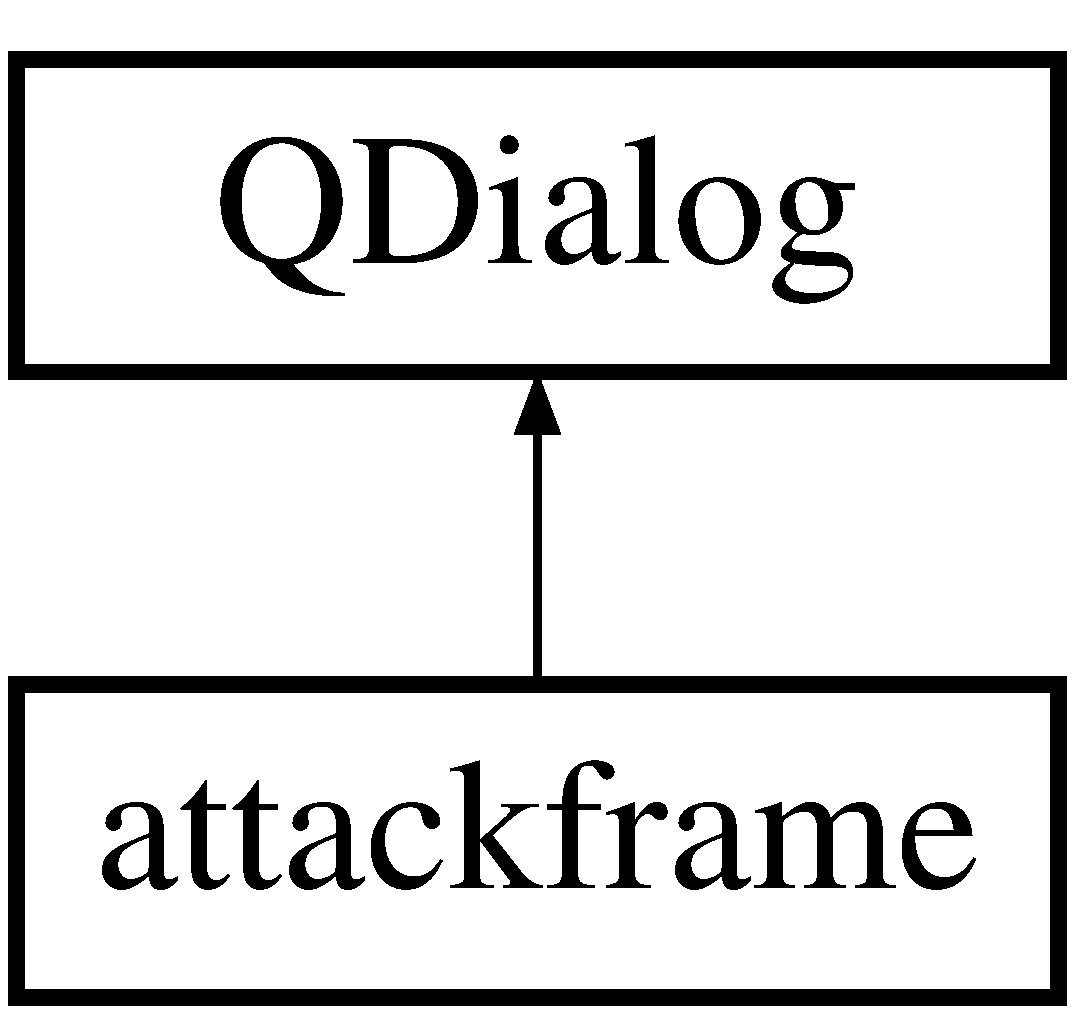
\includegraphics[height=2.000000cm]{classattackframe}
\end{center}
\end{figure}
\subsection*{Public Member Functions}
\begin{DoxyCompactItemize}
\item 
\hypertarget{classattackframe_a4093d85f3f3400f00cca4ffdb87c858d}{{\bfseries attackframe} (Q\-Widget $\ast$parent=0)}\label{classattackframe_a4093d85f3f3400f00cca4ffdb87c858d}

\item 
void \hyperlink{classattackframe_a708bc137367ff5315da0a7f62c1f8494}{start\-Battle} (char etype1, int ehp1, int ex1, int ey1, char etype2, int ehp2, int ex2, int ey2, char etype3, int ehp3, int ex3, int ey3)
\begin{DoxyCompactList}\small\item\em start\-Battle sets up game to fight off enemies \end{DoxyCompactList}\item 
\hyperlink{class_character}{Character} $\ast$ \hyperlink{classattackframe_a1806dca8de141292ba69c8d79609f8d6}{get\-Hero} ()
\begin{DoxyCompactList}\small\item\em get\-Hero method is used to access Hero properties \end{DoxyCompactList}\end{DoxyCompactItemize}
\subsection*{Public Attributes}
\begin{DoxyCompactItemize}
\item 
\hypertarget{classattackframe_a419e0dcfdbae9999b46144a90fff2e37}{int {\bfseries num\-Potions}}\label{classattackframe_a419e0dcfdbae9999b46144a90fff2e37}

\end{DoxyCompactItemize}
\subsection*{Protected Member Functions}
\begin{DoxyCompactItemize}
\item 
\hypertarget{classattackframe_a68df3f4ae2ac6b1a1773d3846cb033cb}{bool {\bfseries event\-Filter} (Q\-Object $\ast$obj, Q\-Event $\ast$event)}\label{classattackframe_a68df3f4ae2ac6b1a1773d3846cb033cb}

\end{DoxyCompactItemize}


\subsection{Member Function Documentation}
\hypertarget{classattackframe_a1806dca8de141292ba69c8d79609f8d6}{\index{attackframe@{attackframe}!get\-Hero@{get\-Hero}}
\index{get\-Hero@{get\-Hero}!attackframe@{attackframe}}
\subsubsection[{get\-Hero}]{\setlength{\rightskip}{0pt plus 5cm}{\bf Character} $\ast$ attackframe\-::get\-Hero (
\begin{DoxyParamCaption}
{}
\end{DoxyParamCaption}
)}}\label{classattackframe_a1806dca8de141292ba69c8d79609f8d6}


get\-Hero method is used to access Hero properties 

\begin{DoxyReturn}{Returns}
pointer to hero 
\end{DoxyReturn}
\hypertarget{classattackframe_a708bc137367ff5315da0a7f62c1f8494}{\index{attackframe@{attackframe}!start\-Battle@{start\-Battle}}
\index{start\-Battle@{start\-Battle}!attackframe@{attackframe}}
\subsubsection[{start\-Battle}]{\setlength{\rightskip}{0pt plus 5cm}void attackframe\-::start\-Battle (
\begin{DoxyParamCaption}
\item[{char}]{etype1, }
\item[{int}]{ehp1, }
\item[{int}]{ex1, }
\item[{int}]{ey1, }
\item[{char}]{etype2, }
\item[{int}]{ehp2, }
\item[{int}]{ex2, }
\item[{int}]{ey2, }
\item[{char}]{etype3, }
\item[{int}]{ehp3, }
\item[{int}]{ex3, }
\item[{int}]{ey3}
\end{DoxyParamCaption}
)}}\label{classattackframe_a708bc137367ff5315da0a7f62c1f8494}


start\-Battle sets up game to fight off enemies 


\begin{DoxyParams}{Parameters}
{\em etype1} & \\
\hline
{\em ehp1} & \\
\hline
{\em ex1} & \\
\hline
{\em ey1} & \\
\hline
{\em etype2} & \\
\hline
{\em ehp2} & \\
\hline
{\em ex2} & \\
\hline
{\em ey2} & \\
\hline
{\em etype3} & \\
\hline
{\em ehp3} & \\
\hline
{\em ex3} & \\
\hline
{\em ey3} & \\
\hline
\end{DoxyParams}


The documentation for this class was generated from the following files\-:\begin{DoxyCompactItemize}
\item 
attackframe.\-h\item 
attackframe.\-cpp\end{DoxyCompactItemize}

\hypertarget{classattack_list}{\section{attack\-List Class Reference}
\label{classattack_list}\index{attack\-List@{attack\-List}}
}
\subsection*{Public Member Functions}
\begin{DoxyCompactItemize}
\item 
\hypertarget{classattack_list_a8bf01a96841205373a2b179c251f6388}{void {\bfseries change\-Move} (int pos, \hyperlink{classattackmove}{attackmove} $\ast$am)}\label{classattack_list_a8bf01a96841205373a2b179c251f6388}

\item 
\hypertarget{classattack_list_acc9d91fc5f10690b2516c123f13f0342}{\hyperlink{classattackmove}{attackmove} $\ast$ {\bfseries get\-Attack} ()}\label{classattack_list_acc9d91fc5f10690b2516c123f13f0342}

\item 
\hypertarget{classattack_list_a40cb4a49c6403918add3cb4a7043788b}{\hyperlink{classattackmove}{attackmove} $\ast$ {\bfseries get\-Attack\-At} (int pos)}\label{classattack_list_a40cb4a49c6403918add3cb4a7043788b}

\item 
\hypertarget{classattack_list_af20e3de4d59258a9e582dc121f0c4bf7}{void {\bfseries add\-Move} (\hyperlink{classattackmove}{attackmove} $\ast$am)}\label{classattack_list_af20e3de4d59258a9e582dc121f0c4bf7}

\item 
\hypertarget{classattack_list_a4efb6e2ae4c3c66b30dbd3e0cc9e330f}{int {\bfseries get\-Curr} ()}\label{classattack_list_a4efb6e2ae4c3c66b30dbd3e0cc9e330f}

\item 
\hypertarget{classattack_list_aef5ebb7304e4f34836a8676398765184}{void {\bfseries reset} ()}\label{classattack_list_aef5ebb7304e4f34836a8676398765184}

\item 
\hypertarget{classattack_list_aa18c2e5fa916658ca18e2d6c94c6fd25}{\hyperlink{classattackmove}{attackmove} $\ast$ {\bfseries take\-Move\-At} (int pos)}\label{classattack_list_aa18c2e5fa916658ca18e2d6c94c6fd25}

\item 
\hypertarget{classattack_list_a251544ca7d79dcaf59e064e6a48480cc}{bool {\bfseries is\-Used\-At} (int pos)}\label{classattack_list_a251544ca7d79dcaf59e064e6a48480cc}

\item 
\hypertarget{classattack_list_a75067d40efdb02cc7011ccd3feb519b9}{int {\bfseries get\-Full} ()}\label{classattack_list_a75067d40efdb02cc7011ccd3feb519b9}

\end{DoxyCompactItemize}


The documentation for this class was generated from the following files\-:\begin{DoxyCompactItemize}
\item 
attacklist.\-h\item 
attacklist.\-cpp\end{DoxyCompactItemize}

\hypertarget{classattackmove}{\section{attackmove Class Reference}
\label{classattackmove}\index{attackmove@{attackmove}}
}
Inheritance diagram for attackmove\-:\begin{figure}[H]
\begin{center}
\leavevmode
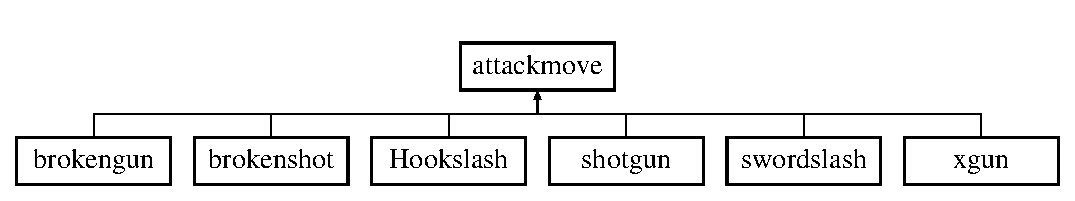
\includegraphics[height=2.000000cm]{classattackmove}
\end{center}
\end{figure}
\subsection*{Public Member Functions}
\begin{DoxyCompactItemize}
\item 
\hypertarget{classattackmove_aeef16b72f9b3b146208a9db33e328b38}{{\bfseries attackmove} (int dam)}\label{classattackmove_aeef16b72f9b3b146208a9db33e328b38}

\item 
\hypertarget{classattackmove_aa971a4aef1cfb1c2ef54301e67e620a6}{int {\bfseries get\-Dam} ()}\label{classattackmove_aa971a4aef1cfb1c2ef54301e67e620a6}

\item 
\hypertarget{classattackmove_a103d4b29b142a466d564de825cf21458}{void {\bfseries set\-Dam} (int dam)}\label{classattackmove_a103d4b29b142a466d564de825cf21458}

\item 
\hypertarget{classattackmove_a80a498f0903dbe791bb1e0faacb54870}{virtual void {\bfseries do\-Attack} (int hpanel, \hyperlink{class_enemy}{Enemy} $\ast$Enemies\mbox{[}3\mbox{]}, \hyperlink{classanim_items}{anim\-Items} $\ast$anim)}\label{classattackmove_a80a498f0903dbe791bb1e0faacb54870}

\item 
\hypertarget{classattackmove_ada49eedf4b893372c576edd48fe73161}{virtual Q\-String {\bfseries get\-String} ()}\label{classattackmove_ada49eedf4b893372c576edd48fe73161}

\item 
\hypertarget{classattackmove_aca59a2343b7a6c195d300dda5c8d952d}{virtual Q\-Image {\bfseries get\-Image} ()}\label{classattackmove_aca59a2343b7a6c195d300dda5c8d952d}

\item 
\hypertarget{classattackmove_a0ff82349551bd72f4d57b3367bb318fa}{virtual void {\bfseries get\-Hover} (int hpanel, \hyperlink{class_enemy}{Enemy} $\ast$Enemies\mbox{[}3\mbox{]}, \hyperlink{classanim_items}{anim\-Items} $\ast$anim)}\label{classattackmove_a0ff82349551bd72f4d57b3367bb318fa}

\end{DoxyCompactItemize}
\subsection*{Protected Attributes}
\begin{DoxyCompactItemize}
\item 
\hypertarget{classattackmove_abeaa53553d9b169032ac273ef2ea7b67}{int {\bfseries damage}}\label{classattackmove_abeaa53553d9b169032ac273ef2ea7b67}

\end{DoxyCompactItemize}


The documentation for this class was generated from the following files\-:\begin{DoxyCompactItemize}
\item 
attackmove.\-h\item 
attackmove.\-cpp\end{DoxyCompactItemize}

\hypertarget{class_battle_pause}{\section{Battle\-Pause Class Reference}
\label{class_battle_pause}\index{Battle\-Pause@{Battle\-Pause}}
}
Inheritance diagram for Battle\-Pause\-:\begin{figure}[H]
\begin{center}
\leavevmode
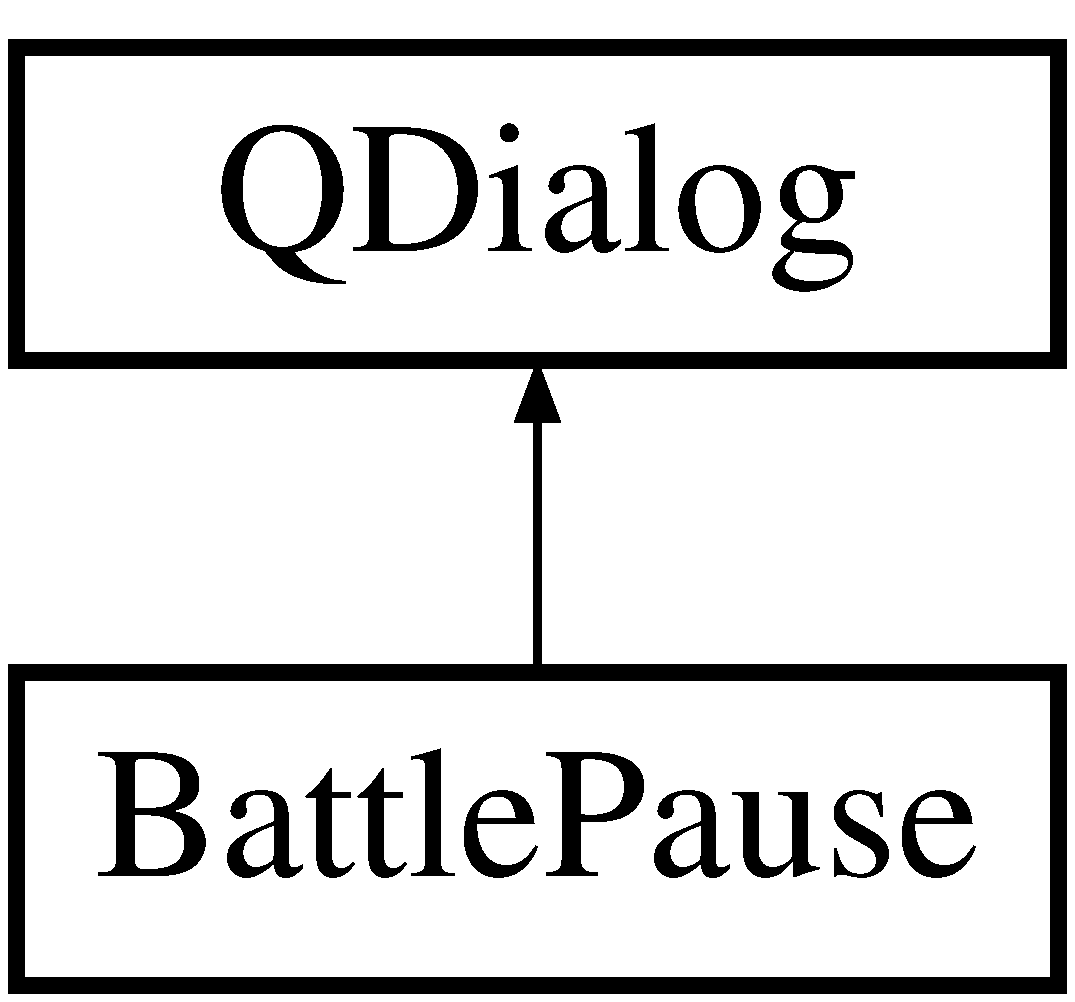
\includegraphics[height=2.000000cm]{class_battle_pause}
\end{center}
\end{figure}
\subsection*{Public Member Functions}
\begin{DoxyCompactItemize}
\item 
\hypertarget{class_battle_pause_a18df0a04e1e6ace26dd944ba5887d65c}{{\bfseries Battle\-Pause} (Q\-Widget $\ast$parent=0)}\label{class_battle_pause_a18df0a04e1e6ace26dd944ba5887d65c}

\end{DoxyCompactItemize}


The documentation for this class was generated from the following files\-:\begin{DoxyCompactItemize}
\item 
battlepause.\-h\item 
battlepause.\-cpp\end{DoxyCompactItemize}

\hypertarget{class_bomber}{\section{Bomber Class Reference}
\label{class_bomber}\index{Bomber@{Bomber}}
}
Inheritance diagram for Bomber\-:\begin{figure}[H]
\begin{center}
\leavevmode
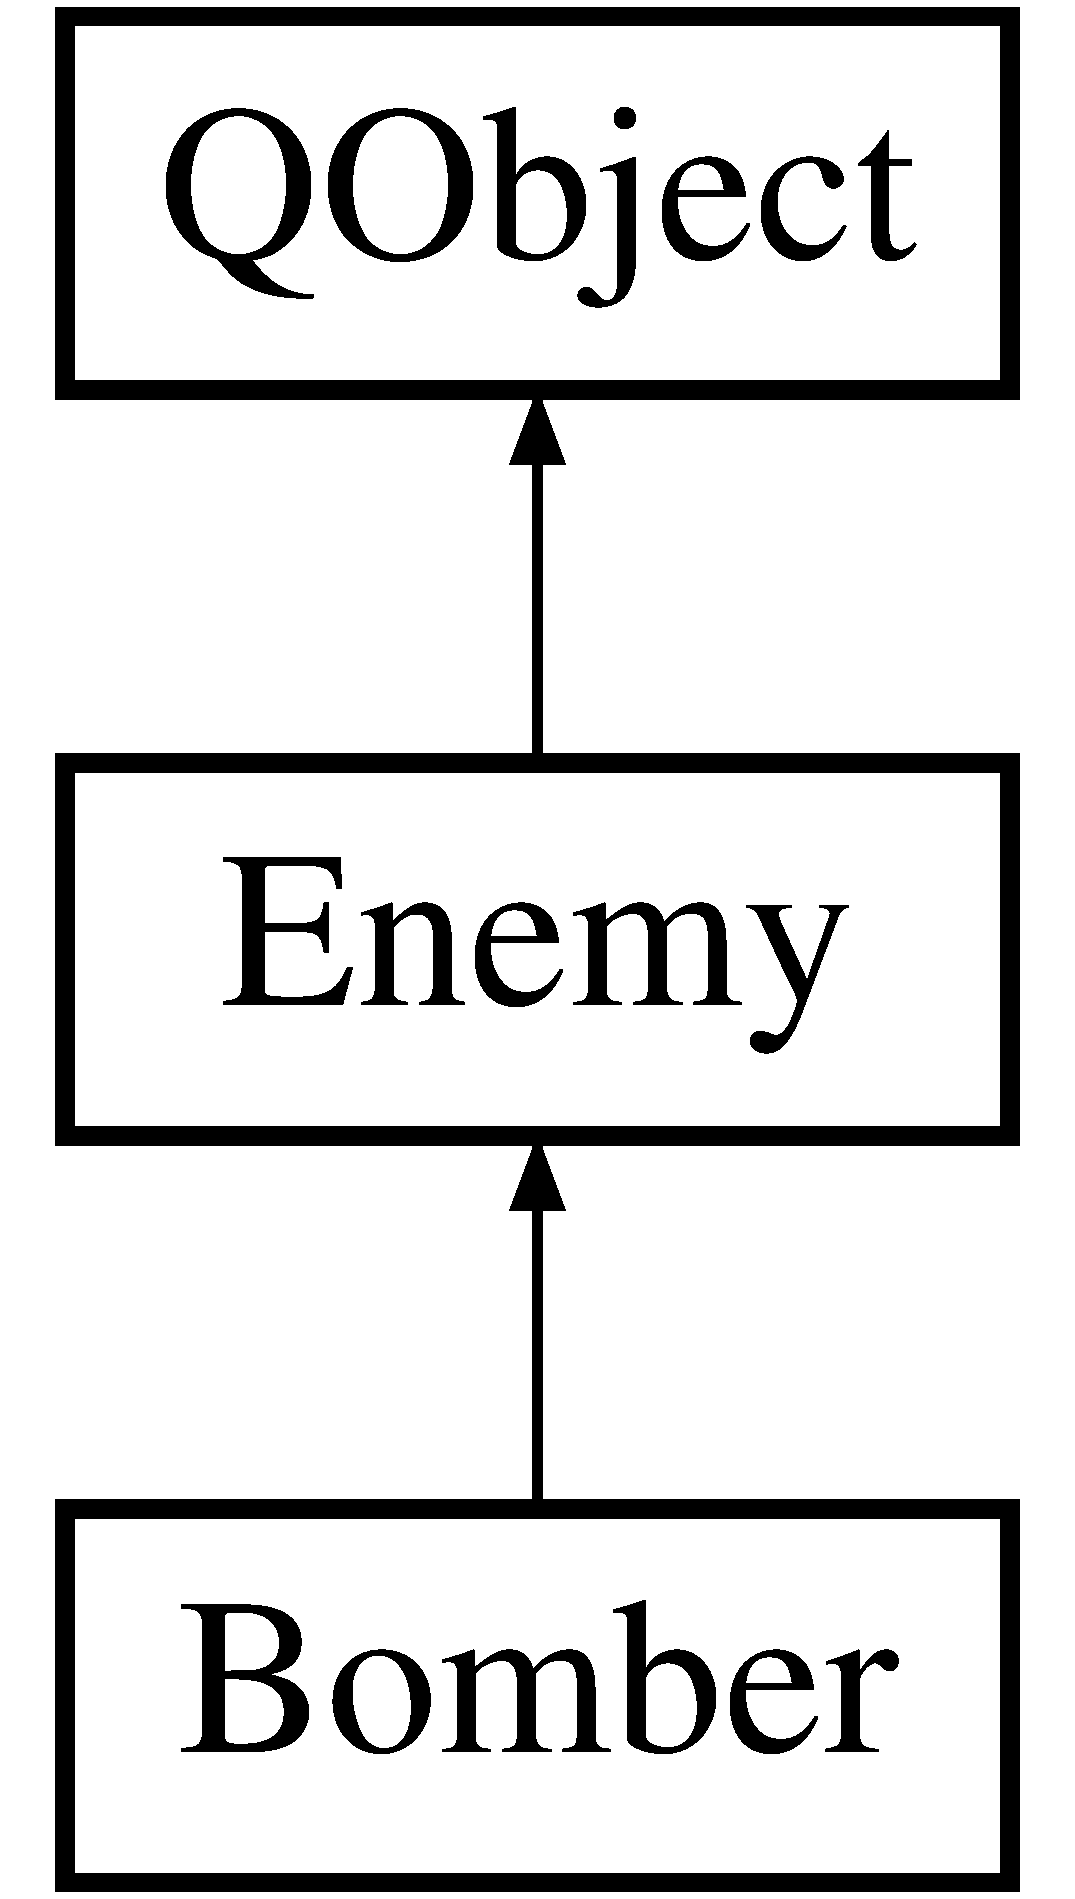
\includegraphics[height=3.000000cm]{class_bomber}
\end{center}
\end{figure}
\subsection*{Public Member Functions}
\begin{DoxyCompactItemize}
\item 
\hypertarget{class_bomber_a69a81ac540c1330e0e6469d236ec5914}{{\bfseries Bomber} (int clev, int cx, int cy)}\label{class_bomber_a69a81ac540c1330e0e6469d236ec5914}

\item 
\hypertarget{class_bomber_ac0f488834e2abdab290699d6efa6e72e}{virtual void {\bfseries do\-Turn} (\hyperlink{class_character}{Character} $\ast$Hero)}\label{class_bomber_ac0f488834e2abdab290699d6efa6e72e}

\item 
\hypertarget{class_bomber_a1ea183ca52092dc27c08f6595072b3a5}{void {\bfseries switch\-Side} ()}\label{class_bomber_a1ea183ca52092dc27c08f6595072b3a5}

\item 
\hypertarget{class_bomber_a500004b8c74a11109bc8174340f3c72d}{void {\bfseries drop\-Bomb} (\hyperlink{class_character}{Character} $\ast$Hero)}\label{class_bomber_a500004b8c74a11109bc8174340f3c72d}

\item 
\hypertarget{class_bomber_af3d20f9c5832eafe7530a22d04294951}{int {\bfseries get\-Ctr} ()}\label{class_bomber_af3d20f9c5832eafe7530a22d04294951}

\item 
\hypertarget{class_bomber_a3b181f6557c19d65adfddb9226a4edfb}{virtual Q\-Image {\bfseries get\-Pic} ()}\label{class_bomber_a3b181f6557c19d65adfddb9226a4edfb}

\item 
\hypertarget{class_bomber_aa75d9256efa7f2996a599deb3db83f90}{virtual void {\bfseries draw\-Self} (Q\-Painter $\ast$g, int gx, int gy)}\label{class_bomber_aa75d9256efa7f2996a599deb3db83f90}

\end{DoxyCompactItemize}
\subsection*{Additional Inherited Members}


The documentation for this class was generated from the following files\-:\begin{DoxyCompactItemize}
\item 
bomber.\-h\item 
bomber.\-cpp\end{DoxyCompactItemize}

\hypertarget{classbrokengun}{\section{brokengun Class Reference}
\label{classbrokengun}\index{brokengun@{brokengun}}
}
Inheritance diagram for brokengun\-:\begin{figure}[H]
\begin{center}
\leavevmode
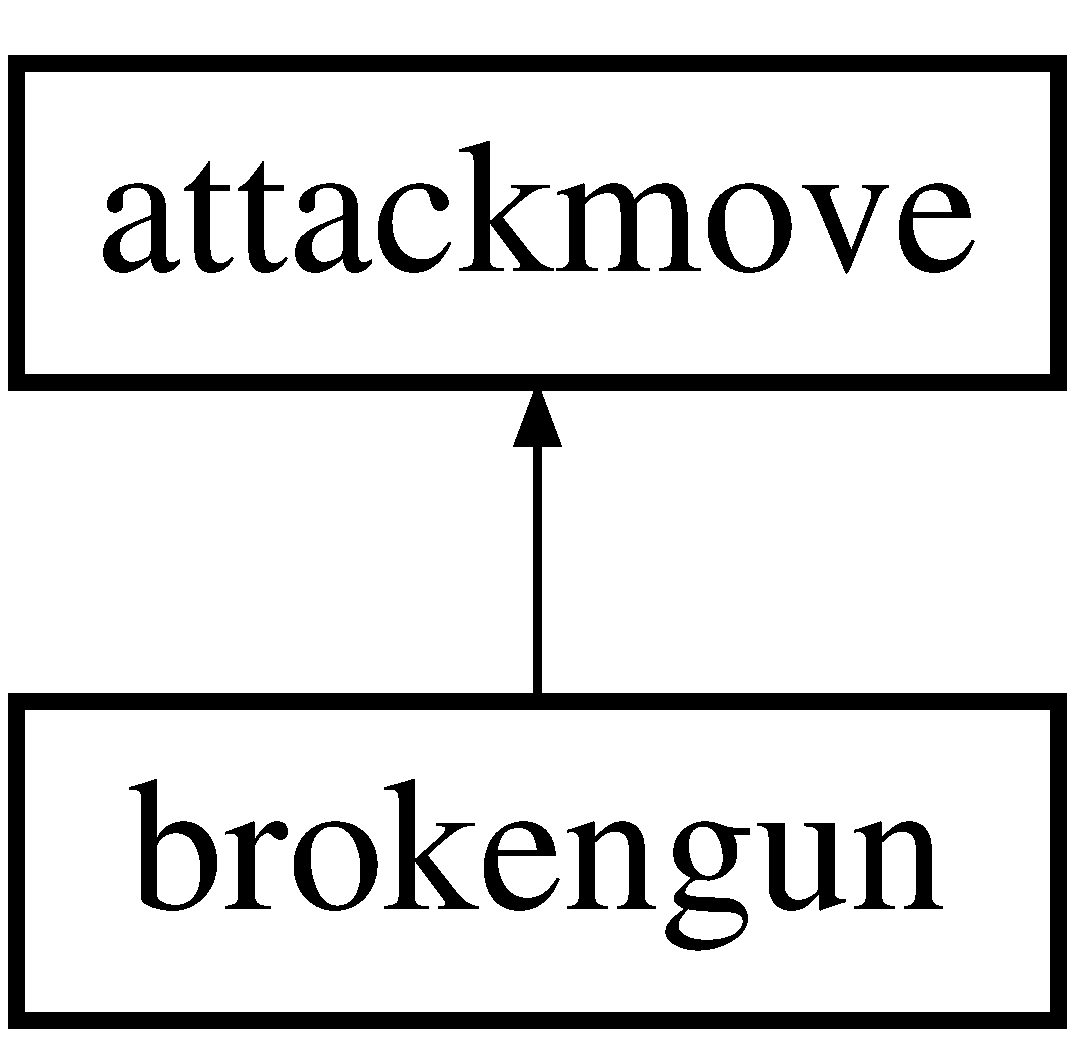
\includegraphics[height=2.000000cm]{classbrokengun}
\end{center}
\end{figure}
\subsection*{Public Member Functions}
\begin{DoxyCompactItemize}
\item 
\hypertarget{classbrokengun_a01e8a685a44e19355ef284c3f172532c}{{\bfseries brokengun} (int dam)}\label{classbrokengun_a01e8a685a44e19355ef284c3f172532c}

\item 
\hypertarget{classbrokengun_af525de1fc249ff4fadec008b367881e9}{virtual Q\-String {\bfseries get\-String} ()}\label{classbrokengun_af525de1fc249ff4fadec008b367881e9}

\item 
\hypertarget{classbrokengun_aceb704b315cbac5e23093637a9b3c0c0}{virtual Q\-Image {\bfseries get\-Image} ()}\label{classbrokengun_aceb704b315cbac5e23093637a9b3c0c0}

\item 
\hypertarget{classbrokengun_ab2250f29c2057006662e77d7f70796d2}{virtual void {\bfseries get\-Hover} (int hpanel, \hyperlink{class_enemy}{Enemy} $\ast$Enemies\mbox{[}3\mbox{]}, \hyperlink{classanim_items}{anim\-Items} $\ast$anim)}\label{classbrokengun_ab2250f29c2057006662e77d7f70796d2}

\item 
\hypertarget{classbrokengun_a36f299faa4df56576af55adbff08a9be}{virtual void {\bfseries do\-Attack} (int hpanel, \hyperlink{class_enemy}{Enemy} $\ast$Enemies\mbox{[}$\,$\mbox{]}, \hyperlink{classanim_items}{anim\-Items} $\ast$anim)}\label{classbrokengun_a36f299faa4df56576af55adbff08a9be}

\end{DoxyCompactItemize}
\subsection*{Additional Inherited Members}


The documentation for this class was generated from the following files\-:\begin{DoxyCompactItemize}
\item 
brokengun.\-h\item 
brokengun.\-cpp\end{DoxyCompactItemize}

\hypertarget{classbrokenshot}{\section{brokenshot Class Reference}
\label{classbrokenshot}\index{brokenshot@{brokenshot}}
}
Inheritance diagram for brokenshot\-:\begin{figure}[H]
\begin{center}
\leavevmode
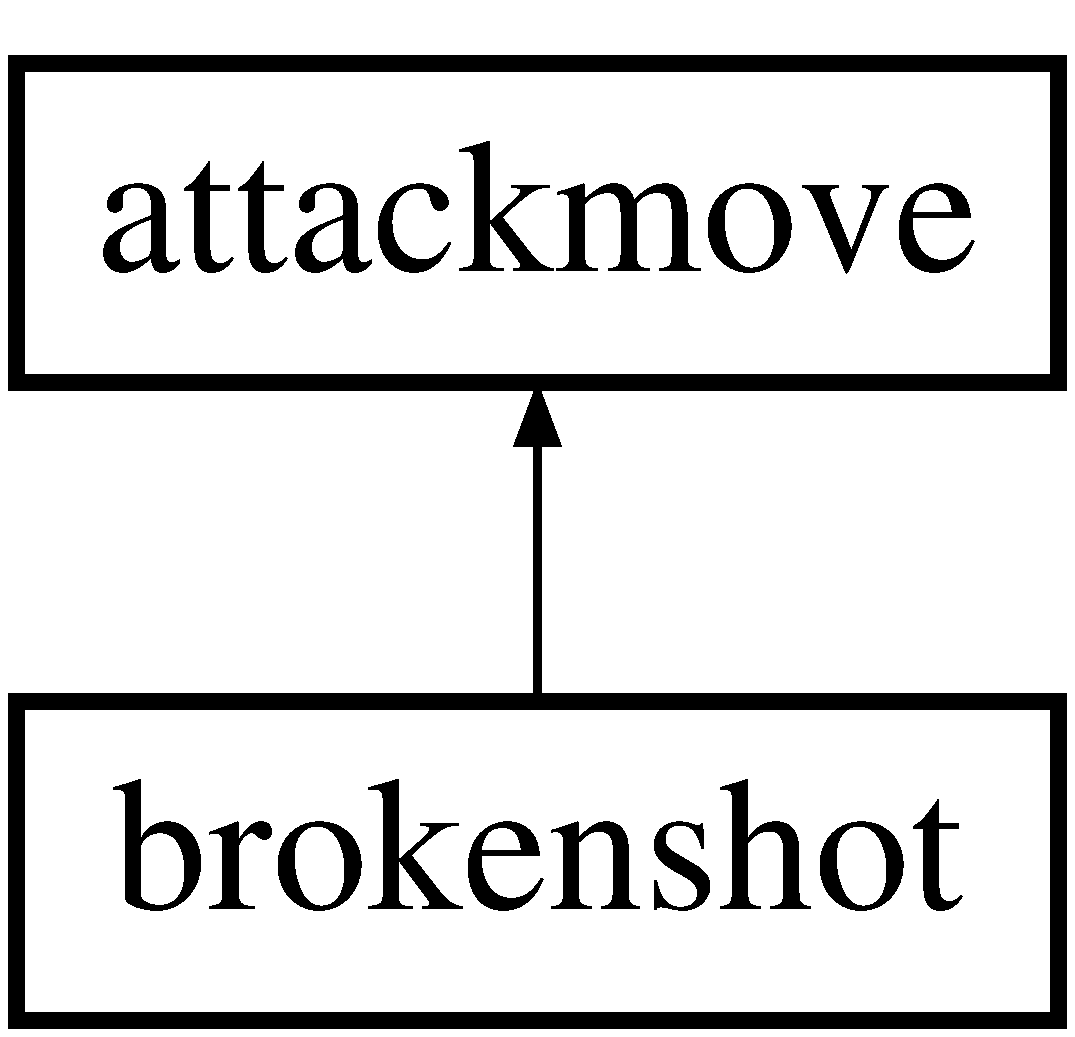
\includegraphics[height=2.000000cm]{classbrokenshot}
\end{center}
\end{figure}
\subsection*{Public Member Functions}
\begin{DoxyCompactItemize}
\item 
\hypertarget{classbrokenshot_aef0d22efead95c42a51a76293cfd91ae}{{\bfseries brokenshot} (int dam)}\label{classbrokenshot_aef0d22efead95c42a51a76293cfd91ae}

\item 
\hypertarget{classbrokenshot_a4834069bb57b3bb17a4816888cc83e43}{virtual Q\-String {\bfseries get\-String} ()}\label{classbrokenshot_a4834069bb57b3bb17a4816888cc83e43}

\item 
\hypertarget{classbrokenshot_ab5a534dcbeb99a57362e22bd11598a27}{virtual Q\-Image {\bfseries get\-Image} ()}\label{classbrokenshot_ab5a534dcbeb99a57362e22bd11598a27}

\item 
\hypertarget{classbrokenshot_a1d9aaa51c4a27d8bb68a8f0678430d3a}{virtual void {\bfseries get\-Hover} (int hpanel, \hyperlink{class_enemy}{Enemy} $\ast$Enemies\mbox{[}3\mbox{]}, \hyperlink{classanim_items}{anim\-Items} $\ast$anim)}\label{classbrokenshot_a1d9aaa51c4a27d8bb68a8f0678430d3a}

\item 
\hypertarget{classbrokenshot_a22b66a06882a1e1761fd796c7548cf50}{virtual void {\bfseries do\-Attack} (int hpanel, \hyperlink{class_enemy}{Enemy} $\ast$Enemies\mbox{[}$\,$\mbox{]}, \hyperlink{classanim_items}{anim\-Items} $\ast$anim)}\label{classbrokenshot_a22b66a06882a1e1761fd796c7548cf50}

\end{DoxyCompactItemize}
\subsection*{Additional Inherited Members}


The documentation for this class was generated from the following files\-:\begin{DoxyCompactItemize}
\item 
brokenshot.\-h\item 
brokenshot.\-cpp\end{DoxyCompactItemize}

\hypertarget{class_cannon}{\section{Cannon Class Reference}
\label{class_cannon}\index{Cannon@{Cannon}}
}
Inheritance diagram for Cannon\-:\begin{figure}[H]
\begin{center}
\leavevmode
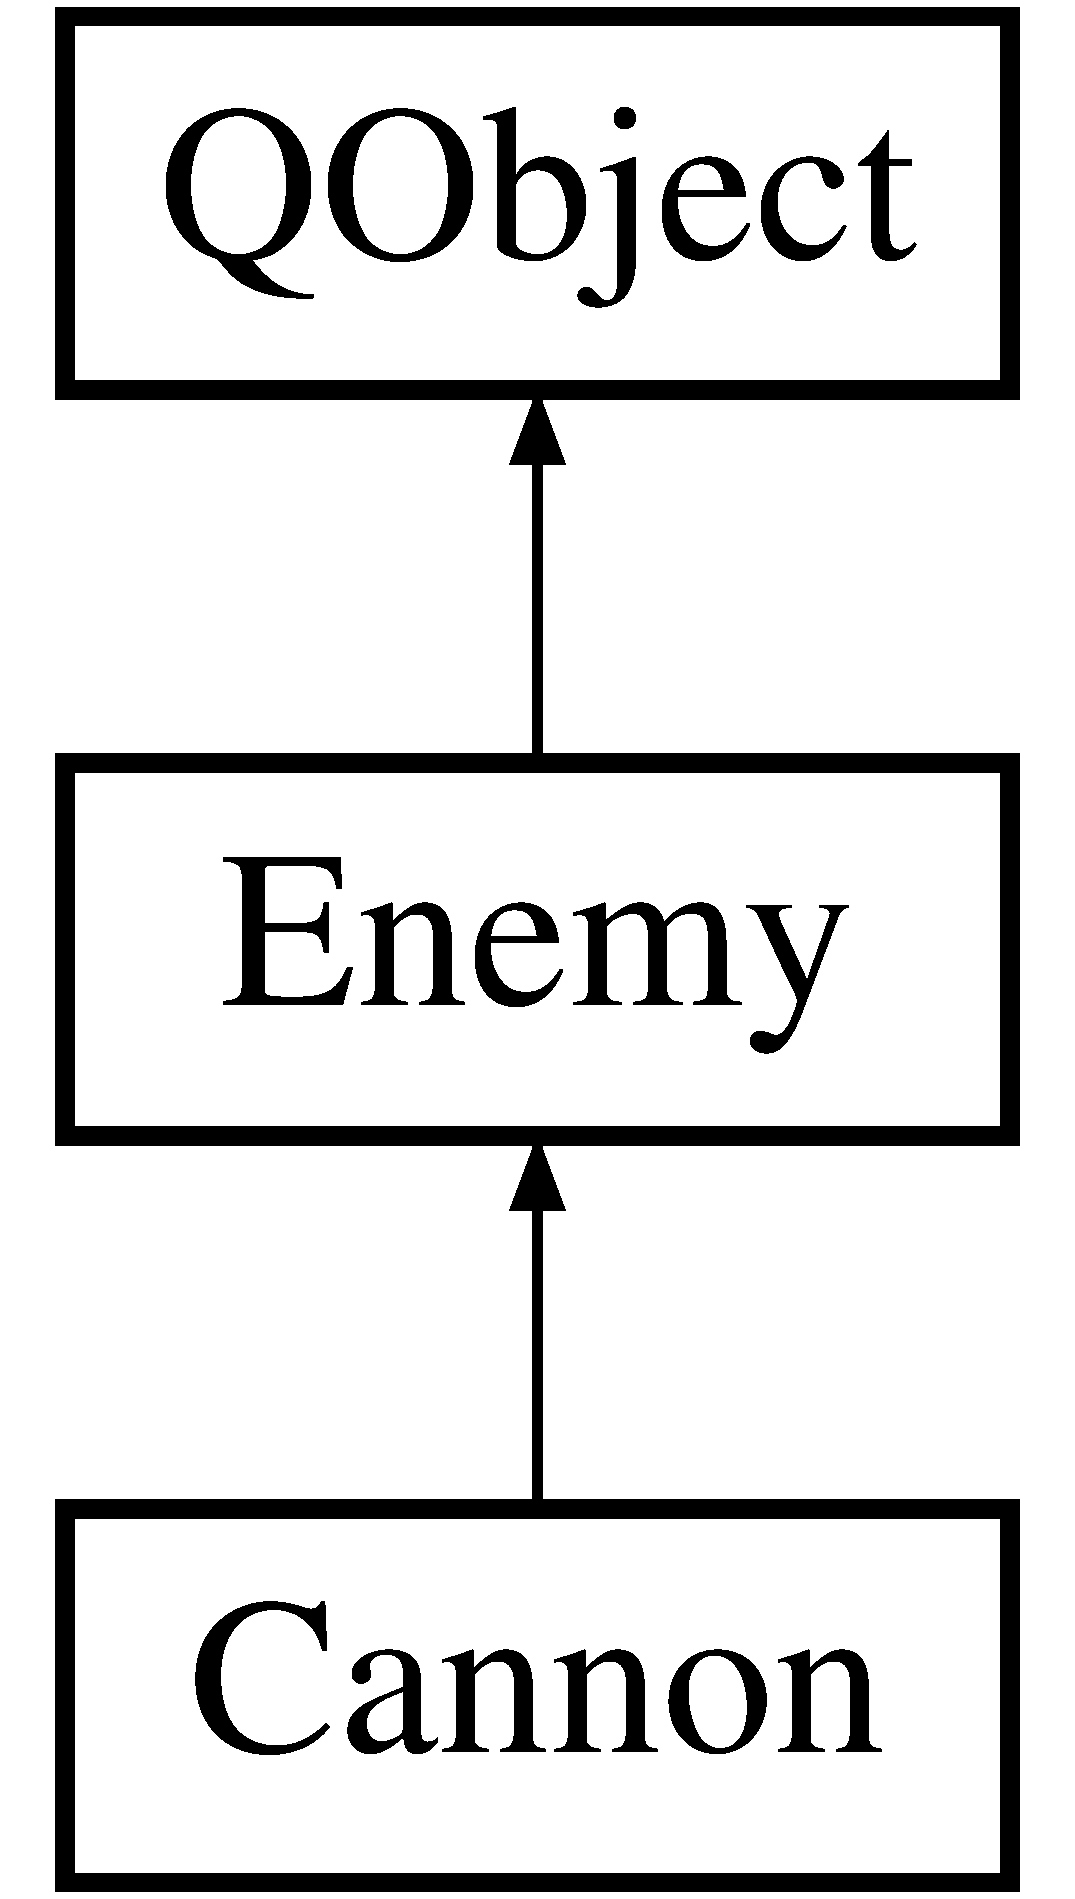
\includegraphics[height=3.000000cm]{class_cannon}
\end{center}
\end{figure}
\subsection*{Public Member Functions}
\begin{DoxyCompactItemize}
\item 
\hypertarget{class_cannon_a167a36b440912282d8c0b44c93afd20d}{{\bfseries Cannon} (int clev, int cx, int cy)}\label{class_cannon_a167a36b440912282d8c0b44c93afd20d}

\item 
\hypertarget{class_cannon_a0ac51832424376a120add27a8b8f2759}{virtual void {\bfseries do\-Turn} (\hyperlink{class_character}{Character} $\ast$Hero)}\label{class_cannon_a0ac51832424376a120add27a8b8f2759}

\item 
\hypertarget{class_cannon_a38f8c0c7f785ee10df1d83c8274ce546}{int {\bfseries get\-Ctr} ()}\label{class_cannon_a38f8c0c7f785ee10df1d83c8274ce546}

\item 
\hypertarget{class_cannon_acd2aee39d3e6b40681c69d44626ce6dd}{virtual Q\-Image {\bfseries get\-Pic} ()}\label{class_cannon_acd2aee39d3e6b40681c69d44626ce6dd}

\item 
\hypertarget{class_cannon_ab3893b885bdc31461a6cacb072b223a3}{virtual void {\bfseries draw\-Self} (Q\-Painter $\ast$g, int gx, int gy)}\label{class_cannon_ab3893b885bdc31461a6cacb072b223a3}

\end{DoxyCompactItemize}
\subsection*{Additional Inherited Members}


The documentation for this class was generated from the following files\-:\begin{DoxyCompactItemize}
\item 
cannon.\-h\item 
cannon.\-cpp\end{DoxyCompactItemize}

\hypertarget{class_character}{\section{Character Class Reference}
\label{class_character}\index{Character@{Character}}
}
\subsection*{Public Member Functions}
\begin{DoxyCompactItemize}
\item 
\hypertarget{class_character_a663231826f9b61c5802228f9b7b743ad}{{\bfseries Character} (int start\-H\-P, int sexp, int cdam, int cpanel)}\label{class_character_a663231826f9b61c5802228f9b7b743ad}

\item 
\hypertarget{class_character_af92b5cb1ab23f30e9aa3371e10e331fe}{bool {\bfseries get\-Damaged} (int damage)}\label{class_character_af92b5cb1ab23f30e9aa3371e10e331fe}

\item 
\hypertarget{class_character_a9e80c446cdcb4651dc321adc80125999}{void {\bfseries get\-Restored} (int recovery)}\label{class_character_a9e80c446cdcb4651dc321adc80125999}

\item 
\hypertarget{class_character_a6f222adddaed0b313094d33700251c6b}{int {\bfseries get\-H\-P} ()}\label{class_character_a6f222adddaed0b313094d33700251c6b}

\item 
\hypertarget{class_character_a0cc4b7dbbaad0f639db856ddfca2e268}{int {\bfseries getexp} ()}\label{class_character_a0cc4b7dbbaad0f639db856ddfca2e268}

\item 
\hypertarget{class_character_a67f56cdab1f01f561073dfcdcf228fda}{int {\bfseries getmax\-H\-P} ()}\label{class_character_a67f56cdab1f01f561073dfcdcf228fda}

\item 
\hypertarget{class_character_a5ee4e596c276d23c486f564c25afe11c}{void {\bfseries set\-H\-P} (int nhp)}\label{class_character_a5ee4e596c276d23c486f564c25afe11c}

\item 
\hypertarget{class_character_afdc04a22ede639e575e6dfc10b15bbcd}{void {\bfseries setexp} (int nexp)}\label{class_character_afdc04a22ede639e575e6dfc10b15bbcd}

\item 
\hypertarget{class_character_ad758a1dde55f9487dccca36ded607a48}{void {\bfseries setmax\-H\-P} (int nmaxhp)}\label{class_character_ad758a1dde55f9487dccca36ded607a48}

\item 
\hypertarget{class_character_ae2ae019ff6d7b8150113fd8add961f39}{void {\bfseries set\-Can\-Move} (bool cmove)}\label{class_character_ae2ae019ff6d7b8150113fd8add961f39}

\item 
\hypertarget{class_character_a5d2616851987d4f844b2c440636f6b7f}{bool {\bfseries get\-Can\-Move} ()}\label{class_character_a5d2616851987d4f844b2c440636f6b7f}

\item 
\hypertarget{class_character_a104dd581ebc631f1b9448abf47d6cb46}{int {\bfseries get\-Panel} ()}\label{class_character_a104dd581ebc631f1b9448abf47d6cb46}

\item 
\hypertarget{class_character_aa3c91db87d4e4ccee3a5bdc9546084de}{void {\bfseries set\-Panel} (int cpanel)}\label{class_character_aa3c91db87d4e4ccee3a5bdc9546084de}

\item 
\hypertarget{class_character_a8173beca9b6a1aee4213156f44f73708}{void {\bfseries set\-Turn} (bool cturn)}\label{class_character_a8173beca9b6a1aee4213156f44f73708}

\item 
\hypertarget{class_character_afad175e9eb494ea86fb3f3f03becbf86}{bool {\bfseries is\-Turn} ()}\label{class_character_afad175e9eb494ea86fb3f3f03becbf86}

\item 
\hypertarget{class_character_ae5614f09a48cab021451e1d174c49f40}{void {\bfseries set\-Dam} (int cdam)}\label{class_character_ae5614f09a48cab021451e1d174c49f40}

\item 
\hypertarget{class_character_a22e0b2d268c078a0a2055bc547c13779}{int {\bfseries get\-Dam} ()}\label{class_character_a22e0b2d268c078a0a2055bc547c13779}

\item 
\hypertarget{class_character_af20f9fcc4dc0439c3d33463d52f62baa}{int {\bfseries get\-Gold} ()}\label{class_character_af20f9fcc4dc0439c3d33463d52f62baa}

\item 
\hypertarget{class_character_a022b611a56f1c4a87972de352b9c58ed}{void {\bfseries inc\-Gold} (int amt)}\label{class_character_a022b611a56f1c4a87972de352b9c58ed}

\end{DoxyCompactItemize}


The documentation for this class was generated from the following files\-:\begin{DoxyCompactItemize}
\item 
character.\-h\item 
character.\-cpp\end{DoxyCompactItemize}

\hypertarget{class_enemy}{\section{Enemy Class Reference}
\label{class_enemy}\index{Enemy@{Enemy}}
}
Inheritance diagram for Enemy\-:\begin{figure}[H]
\begin{center}
\leavevmode
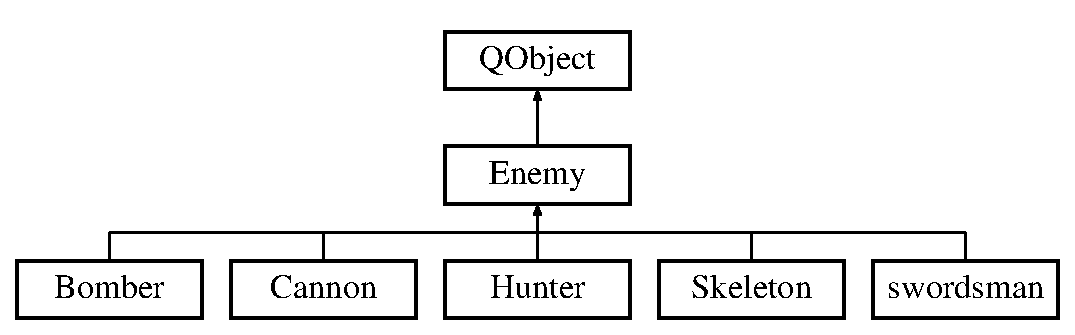
\includegraphics[height=3.000000cm]{class_enemy}
\end{center}
\end{figure}
\subsection*{Public Member Functions}
\begin{DoxyCompactItemize}
\item 
\hypertarget{class_enemy_a0638b6e9f11a72831051438dbf803d91}{{\bfseries Enemy} (int clev, int cx, int cy)}\label{class_enemy_a0638b6e9f11a72831051438dbf803d91}

\item 
\hypertarget{class_enemy_a0ebc35bd4cd41e81df912b6286426c46}{void {\bfseries set\-X} (int cx)}\label{class_enemy_a0ebc35bd4cd41e81df912b6286426c46}

\item 
\hypertarget{class_enemy_a1fab961fbc5b1fd1764515c1a00f424b}{void {\bfseries set\-Y} (int cy)}\label{class_enemy_a1fab961fbc5b1fd1764515c1a00f424b}

\item 
\hypertarget{class_enemy_aa07b45a0163d1c16326dc8706ec77414}{void {\bfseries set\-Turn} (bool cmove)}\label{class_enemy_aa07b45a0163d1c16326dc8706ec77414}

\item 
\hypertarget{class_enemy_a8742266192bffefd0746d5665e816463}{void {\bfseries set\-Move} (bool cmove)}\label{class_enemy_a8742266192bffefd0746d5665e816463}

\item 
\hypertarget{class_enemy_abdd71d2a54bf169ffb71801091704881}{int {\bfseries get\-X} ()}\label{class_enemy_abdd71d2a54bf169ffb71801091704881}

\item 
\hypertarget{class_enemy_a056667d7235d861cdc88ecfe2341ca90}{int {\bfseries get\-Y} ()}\label{class_enemy_a056667d7235d861cdc88ecfe2341ca90}

\item 
\hypertarget{class_enemy_a742cf2ff493fd15a4a11a13e20e60423}{bool {\bfseries get\-Move} ()}\label{class_enemy_a742cf2ff493fd15a4a11a13e20e60423}

\item 
\hypertarget{class_enemy_ad25491cf4bd75217a4d97318f0ec0677}{bool {\bfseries get\-Turn} ()}\label{class_enemy_ad25491cf4bd75217a4d97318f0ec0677}

\item 
\hypertarget{class_enemy_ab1c5ecbd2567b509a5d4492764a28f5d}{int {\bfseries get\-H\-P} ()}\label{class_enemy_ab1c5ecbd2567b509a5d4492764a28f5d}

\item 
\hypertarget{class_enemy_a32c6b8b1784ff8301c1cb20d969bb6bb}{int {\bfseries getmax\-H\-P} ()}\label{class_enemy_a32c6b8b1784ff8301c1cb20d969bb6bb}

\item 
\hypertarget{class_enemy_a4c6c4bfd244315ba6cfd338428f33d48}{bool {\bfseries get\-Alive} ()}\label{class_enemy_a4c6c4bfd244315ba6cfd338428f33d48}

\item 
\hypertarget{class_enemy_aa9ed76dea0526fba28e15e9667a9eb25}{void {\bfseries set\-Alive} (bool is\-Alive)}\label{class_enemy_aa9ed76dea0526fba28e15e9667a9eb25}

\item 
\hypertarget{class_enemy_a56e4b9b07e8cd2a4e5ecfa8ff5b9265a}{virtual void {\bfseries do\-Turn} (\hyperlink{class_character}{Character} $\ast$Hero)}\label{class_enemy_a56e4b9b07e8cd2a4e5ecfa8ff5b9265a}

\item 
\hypertarget{class_enemy_a577a10f1cd0eb2bdd7f600c63044b010}{bool {\bfseries get\-Damaged} (int damage)}\label{class_enemy_a577a10f1cd0eb2bdd7f600c63044b010}

\item 
\hypertarget{class_enemy_a17b20f01b5af2ca88c844fb0f072f4fc}{void {\bfseries get\-Restored} (int recovery)}\label{class_enemy_a17b20f01b5af2ca88c844fb0f072f4fc}

\item 
\hypertarget{class_enemy_a7eb85dffc1f22c21eb6ff805192f3818}{virtual Q\-Image {\bfseries get\-Pic} ()}\label{class_enemy_a7eb85dffc1f22c21eb6ff805192f3818}

\item 
\hypertarget{class_enemy_a3251244e8e7ac657687d6be5a8da71bb}{virtual void {\bfseries draw\-Self} (Q\-Painter $\ast$g, int gx, int gy)}\label{class_enemy_a3251244e8e7ac657687d6be5a8da71bb}

\end{DoxyCompactItemize}
\subsection*{Protected Attributes}
\begin{DoxyCompactItemize}
\item 
\hypertarget{class_enemy_ab685146410b2972ccab930a522fd9252}{int {\bfseries xpos}}\label{class_enemy_ab685146410b2972ccab930a522fd9252}

\item 
\hypertarget{class_enemy_a7cb1bc241abdacc846ae2313f2a54bbc}{int {\bfseries ypos}}\label{class_enemy_a7cb1bc241abdacc846ae2313f2a54bbc}

\item 
\hypertarget{class_enemy_a2891f607bd7c05774ab7efaf155c1842}{int {\bfseries current\-H\-P}}\label{class_enemy_a2891f607bd7c05774ab7efaf155c1842}

\item 
\hypertarget{class_enemy_a990ecf4cbfdae850b51e6fb2b367ad8e}{int {\bfseries max\-H\-P}}\label{class_enemy_a990ecf4cbfdae850b51e6fb2b367ad8e}

\item 
\hypertarget{class_enemy_a09d68a627f0f664d0dd3ac8063dd5cb3}{int {\bfseries in\-Turn}}\label{class_enemy_a09d68a627f0f664d0dd3ac8063dd5cb3}

\item 
\hypertarget{class_enemy_a5bbd6ff8c998dc4a67badee154c9e453}{int {\bfseries canmove}}\label{class_enemy_a5bbd6ff8c998dc4a67badee154c9e453}

\item 
\hypertarget{class_enemy_a02481d9c8d5b64d4d83556e047fcda7b}{bool {\bfseries Alive}}\label{class_enemy_a02481d9c8d5b64d4d83556e047fcda7b}

\item 
\hypertarget{class_enemy_a4754b00e9ff05f83a293f74324016c17}{int {\bfseries level}}\label{class_enemy_a4754b00e9ff05f83a293f74324016c17}

\item 
\hypertarget{class_enemy_a4969f2e5372ae6840aba5cd0b8059a0a}{int {\bfseries damage}}\label{class_enemy_a4969f2e5372ae6840aba5cd0b8059a0a}

\end{DoxyCompactItemize}


The documentation for this class was generated from the following files\-:\begin{DoxyCompactItemize}
\item 
enemy.\-h\item 
enemy.\-cpp\end{DoxyCompactItemize}

\hypertarget{class_hookslash}{\section{Hookslash Class Reference}
\label{class_hookslash}\index{Hookslash@{Hookslash}}
}
Inheritance diagram for Hookslash\-:\begin{figure}[H]
\begin{center}
\leavevmode
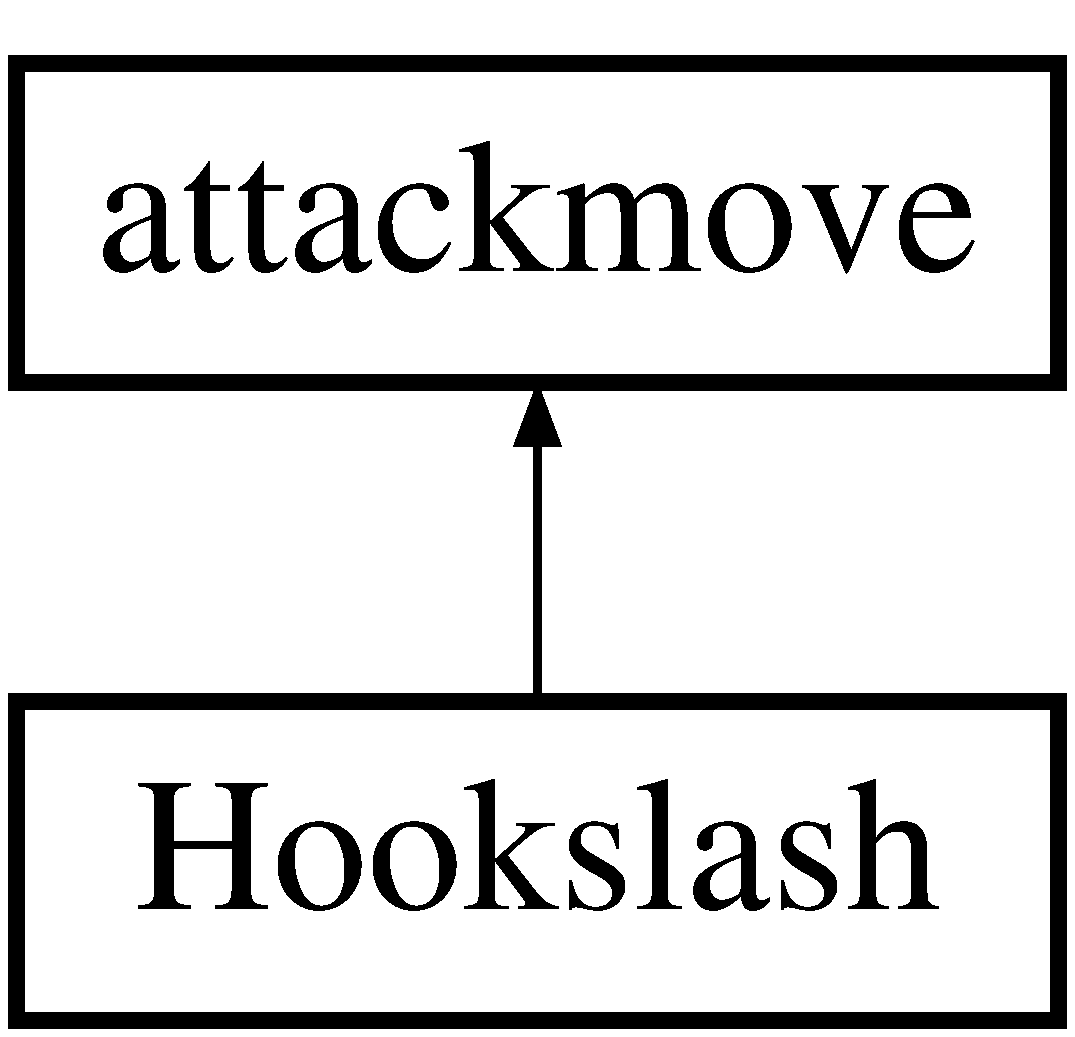
\includegraphics[height=2.000000cm]{class_hookslash}
\end{center}
\end{figure}
\subsection*{Public Member Functions}
\begin{DoxyCompactItemize}
\item 
\hypertarget{class_hookslash_a70ac467f48108a4fe26e4db666b217f8}{{\bfseries Hookslash} (int dam)}\label{class_hookslash_a70ac467f48108a4fe26e4db666b217f8}

\item 
\hypertarget{class_hookslash_aaf31aabb624b138d98f3c94fe1c37fcc}{virtual Q\-String {\bfseries get\-String} ()}\label{class_hookslash_aaf31aabb624b138d98f3c94fe1c37fcc}

\item 
\hypertarget{class_hookslash_a65c6e01ac90d1f01139dd08b93aeaa0a}{virtual Q\-Image {\bfseries get\-Image} ()}\label{class_hookslash_a65c6e01ac90d1f01139dd08b93aeaa0a}

\item 
\hypertarget{class_hookslash_ab6a6ca9582c4d8dad26b481292bca6a0}{virtual void {\bfseries get\-Hover} (int hpanel, \hyperlink{class_enemy}{Enemy} $\ast$Enemies\mbox{[}3\mbox{]}, \hyperlink{classanim_items}{anim\-Items} $\ast$anim)}\label{class_hookslash_ab6a6ca9582c4d8dad26b481292bca6a0}

\item 
\hypertarget{class_hookslash_a704f02d57c898d1256c260218fe5c359}{virtual void {\bfseries do\-Attack} (int hpanel, \hyperlink{class_enemy}{Enemy} $\ast$Enemies\mbox{[}$\,$\mbox{]}, \hyperlink{classanim_items}{anim\-Items} $\ast$anim)}\label{class_hookslash_a704f02d57c898d1256c260218fe5c359}

\end{DoxyCompactItemize}
\subsection*{Additional Inherited Members}


The documentation for this class was generated from the following files\-:\begin{DoxyCompactItemize}
\item 
hookslash.\-h\item 
hookslash.\-cpp\end{DoxyCompactItemize}

\hypertarget{class_hunter}{\section{Hunter Class Reference}
\label{class_hunter}\index{Hunter@{Hunter}}
}
Inheritance diagram for Hunter\-:\begin{figure}[H]
\begin{center}
\leavevmode
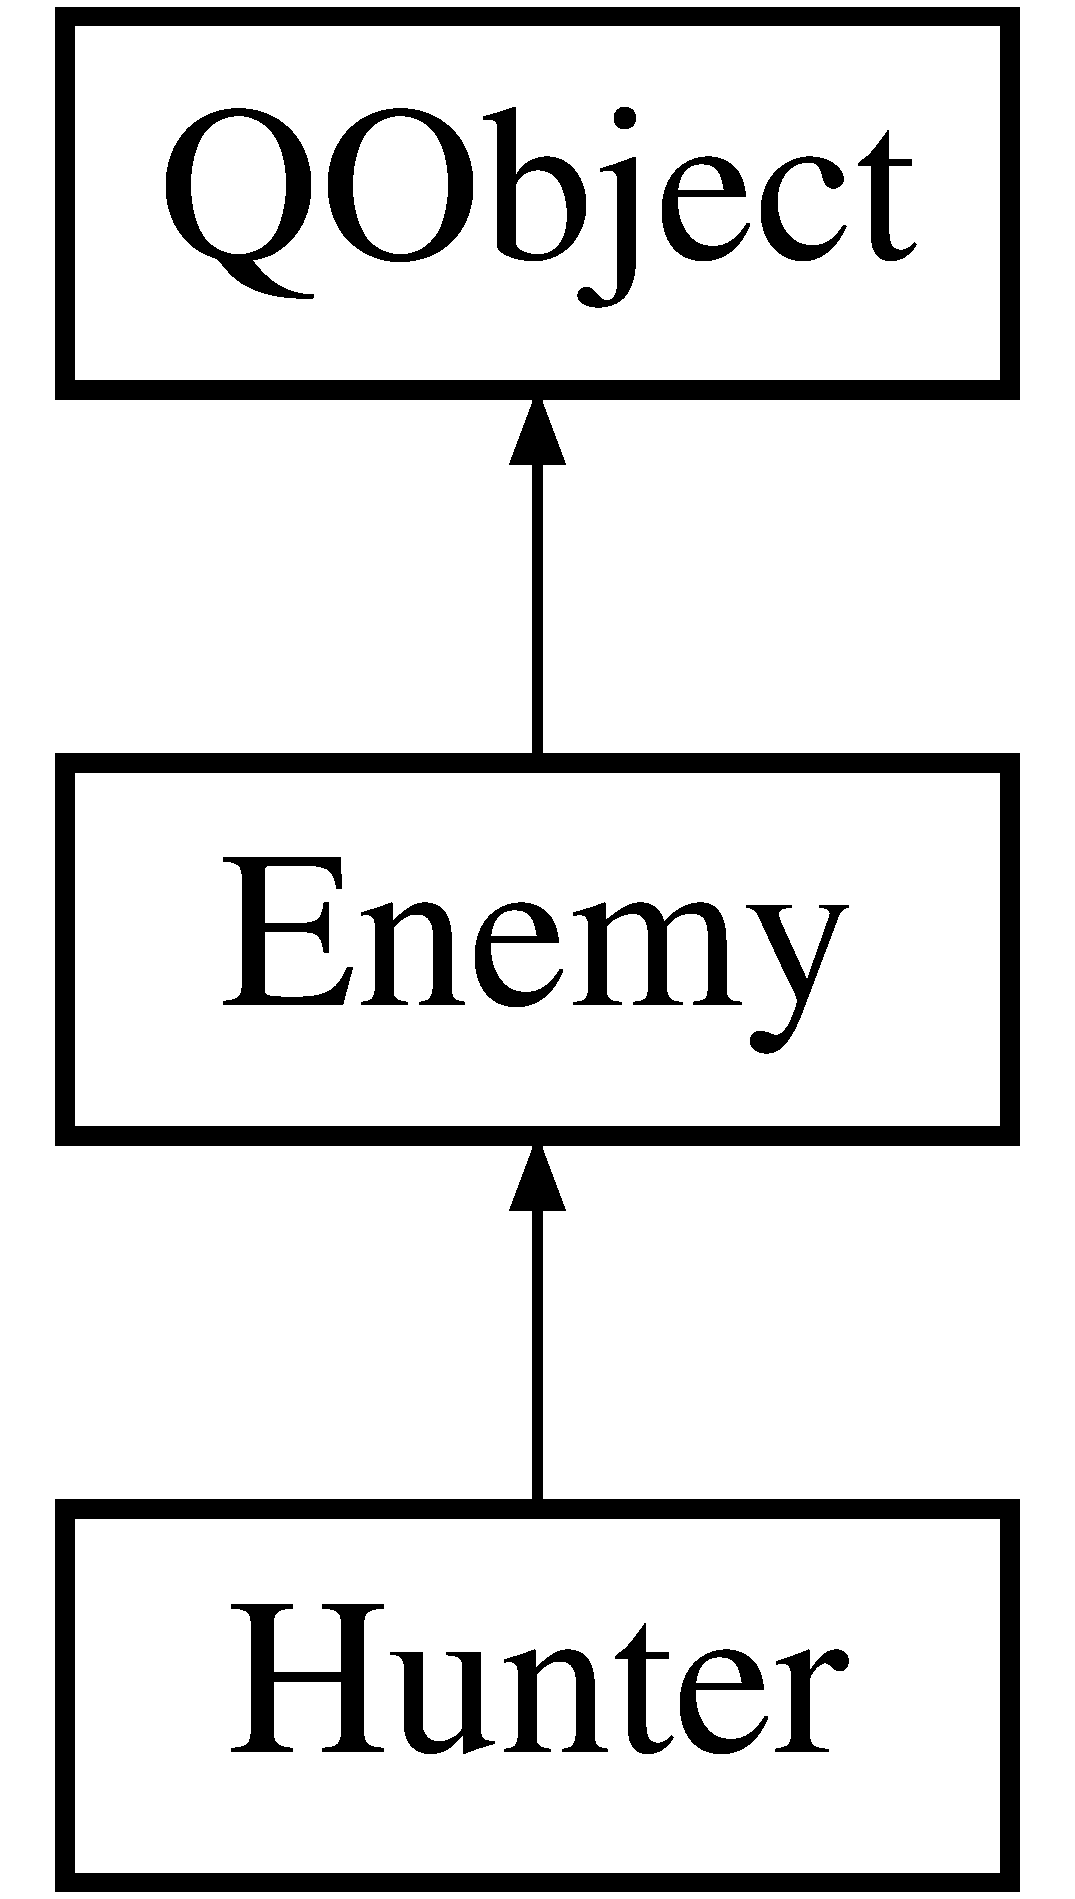
\includegraphics[height=3.000000cm]{class_hunter}
\end{center}
\end{figure}
\subsection*{Public Member Functions}
\begin{DoxyCompactItemize}
\item 
\hypertarget{class_hunter_a6516ea26662db6188fa2102ae768eca2}{{\bfseries Hunter} (int clev, int cx, int cy, bool cup)}\label{class_hunter_a6516ea26662db6188fa2102ae768eca2}

\item 
\hypertarget{class_hunter_a910f2c34961a3d7fb1caa91e65b5d743}{virtual void {\bfseries do\-Turn} (\hyperlink{class_character}{Character} $\ast$Hero)}\label{class_hunter_a910f2c34961a3d7fb1caa91e65b5d743}

\item 
\hypertarget{class_hunter_adc1727098c026b726430a638d4536970}{bool {\bfseries get\-Lef} ()}\label{class_hunter_adc1727098c026b726430a638d4536970}

\item 
\hypertarget{class_hunter_ac1cb95a730a5af30d4fe50b1ff296696}{void {\bfseries set\-Lef} (bool clef)}\label{class_hunter_ac1cb95a730a5af30d4fe50b1ff296696}

\item 
\hypertarget{class_hunter_a407e130c2e904630fd501c329eaeac77}{virtual Q\-Image {\bfseries get\-Pic} ()}\label{class_hunter_a407e130c2e904630fd501c329eaeac77}

\item 
\hypertarget{class_hunter_a765f282edf2fd27998740d33ed81a423}{virtual void {\bfseries draw\-Self} (Q\-Painter $\ast$g, int gx, int gy)}\label{class_hunter_a765f282edf2fd27998740d33ed81a423}

\end{DoxyCompactItemize}
\subsection*{Additional Inherited Members}


The documentation for this class was generated from the following files\-:\begin{DoxyCompactItemize}
\item 
hunter.\-h\item 
hunter.\-cpp\end{DoxyCompactItemize}

\hypertarget{class_main_window}{\section{Main\-Window Class Reference}
\label{class_main_window}\index{Main\-Window@{Main\-Window}}
}
Inheritance diagram for Main\-Window\-:\begin{figure}[H]
\begin{center}
\leavevmode
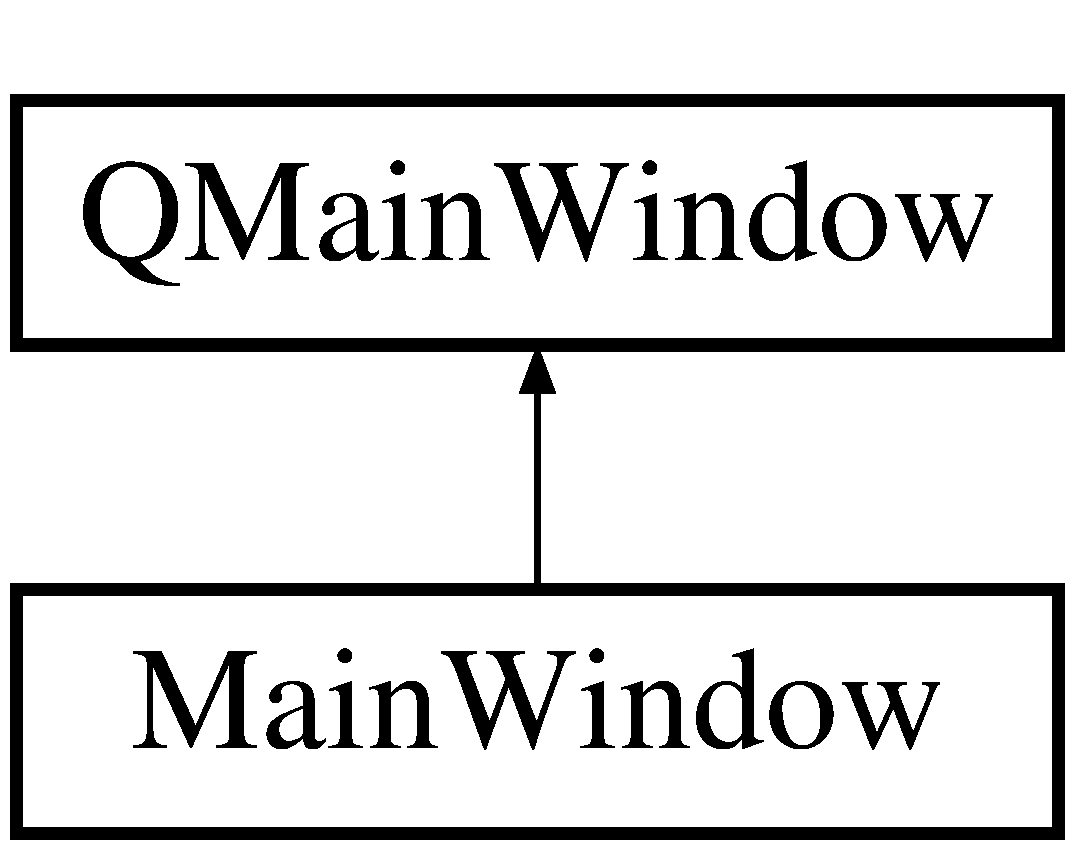
\includegraphics[height=2.000000cm]{class_main_window}
\end{center}
\end{figure}
\subsection*{Public Member Functions}
\begin{DoxyCompactItemize}
\item 
\hypertarget{class_main_window_a8b244be8b7b7db1b08de2a2acb9409db}{{\bfseries Main\-Window} (Q\-Widget $\ast$parent=0)}\label{class_main_window_a8b244be8b7b7db1b08de2a2acb9409db}

\end{DoxyCompactItemize}


The documentation for this class was generated from the following files\-:\begin{DoxyCompactItemize}
\item 
mainwindow.\-h\item 
mainwindow.\-cpp\end{DoxyCompactItemize}

\hypertarget{class_map_enemy}{\section{Map\-Enemy Class Reference}
\label{class_map_enemy}\index{Map\-Enemy@{Map\-Enemy}}
}
Inheritance diagram for Map\-Enemy\-:\begin{figure}[H]
\begin{center}
\leavevmode
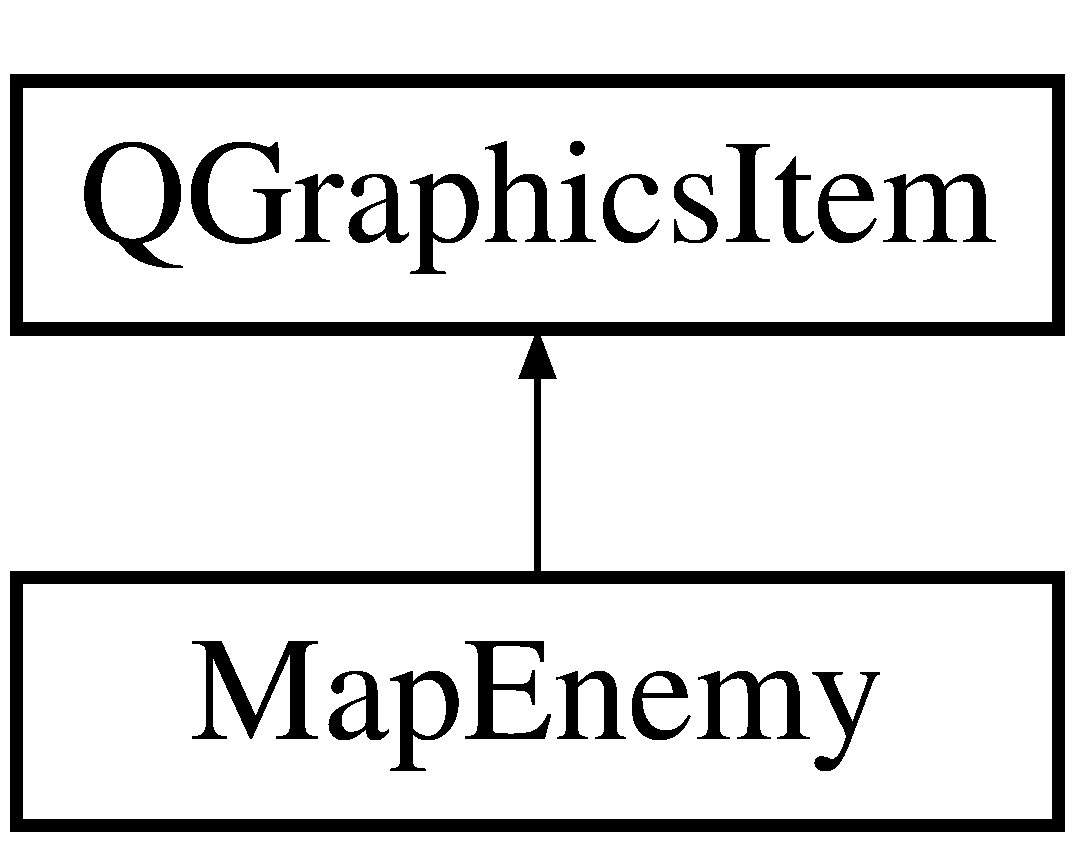
\includegraphics[height=2.000000cm]{class_map_enemy}
\end{center}
\end{figure}
\subsection*{Public Member Functions}
\begin{DoxyCompactItemize}
\item 
\hypertarget{class_map_enemy_a0ec0658d11120c1618bdd39fae1c8f30}{{\bfseries Map\-Enemy} (Q\-Graphics\-Item $\ast$parent=N\-U\-L\-L)}\label{class_map_enemy_a0ec0658d11120c1618bdd39fae1c8f30}

\end{DoxyCompactItemize}
\subsection*{Protected Member Functions}
\begin{DoxyCompactItemize}
\item 
\hypertarget{class_map_enemy_a824c6d66bce423f3e89fe4111a9cf2f0}{void {\bfseries paint} (Q\-Painter $\ast$painter, const Q\-Style\-Option\-Graphics\-Item $\ast$option, Q\-Widget $\ast$widget)}\label{class_map_enemy_a824c6d66bce423f3e89fe4111a9cf2f0}

\item 
\hypertarget{class_map_enemy_ae8847f947b045ae9fd3c1fd7ccb522fc}{Q\-Rect\-F {\bfseries bounding\-Rect} () const }\label{class_map_enemy_ae8847f947b045ae9fd3c1fd7ccb522fc}

\item 
\hypertarget{class_map_enemy_a8b41e9638d4c20b9480b6e1130510bf8}{virtual void {\bfseries collision\-Event} ()}\label{class_map_enemy_a8b41e9638d4c20b9480b6e1130510bf8}

\end{DoxyCompactItemize}


The documentation for this class was generated from the following files\-:\begin{DoxyCompactItemize}
\item 
mapenemy.\-h\item 
mapenemy.\-cpp\end{DoxyCompactItemize}

\hypertarget{class_map_hero}{\section{Map\-Hero Class Reference}
\label{class_map_hero}\index{Map\-Hero@{Map\-Hero}}
}
Inheritance diagram for Map\-Hero\-:\begin{figure}[H]
\begin{center}
\leavevmode
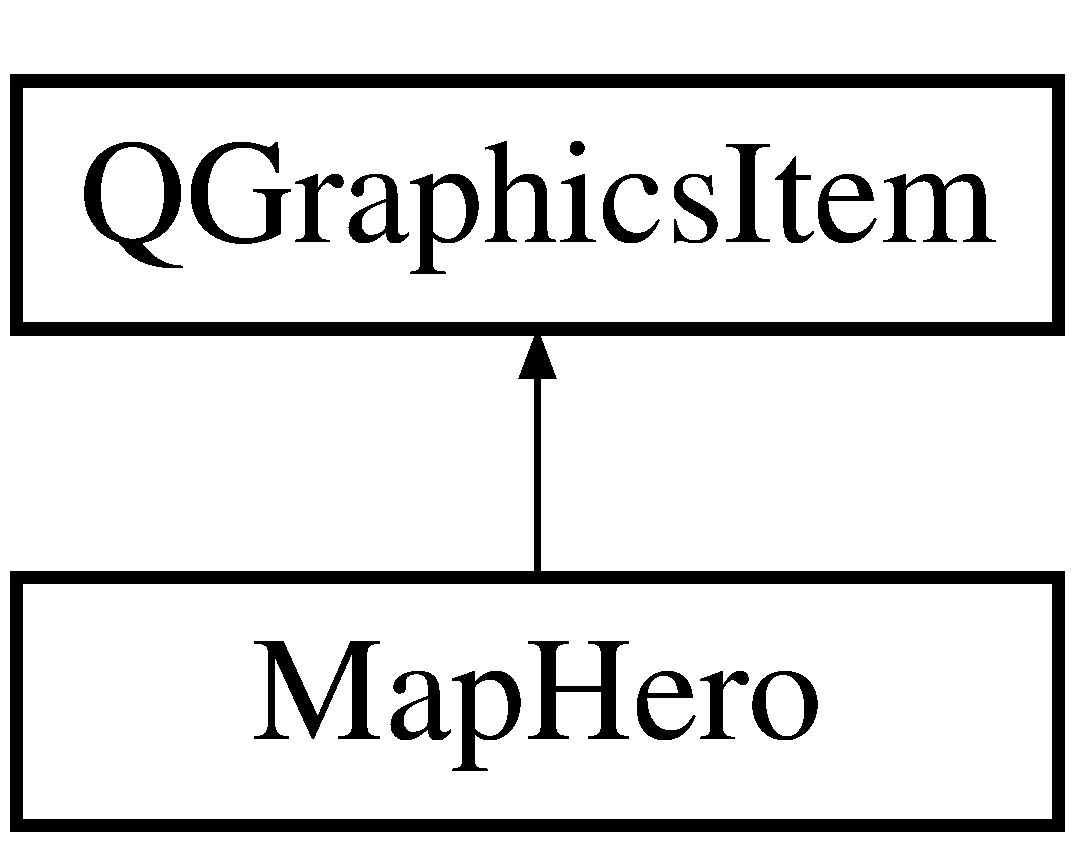
\includegraphics[height=2.000000cm]{class_map_hero}
\end{center}
\end{figure}
\subsection*{Public Member Functions}
\begin{DoxyCompactItemize}
\item 
\hypertarget{class_map_hero_aa5dd4f5162b14b9c4dca9fe6b53482bd}{{\bfseries Map\-Hero} (Q\-Graphics\-Item $\ast$parent=0)}\label{class_map_hero_aa5dd4f5162b14b9c4dca9fe6b53482bd}

\item 
\hypertarget{class_map_hero_a8337402793f86be45d7b139b328f4f81}{void {\bfseries point\-To\-Enemy} (\hyperlink{class_map_enemy}{Map\-Enemy} $\ast$enemy)}\label{class_map_hero_a8337402793f86be45d7b139b328f4f81}

\end{DoxyCompactItemize}
\subsection*{Public Attributes}
\begin{DoxyCompactItemize}
\item 
\hypertarget{class_map_hero_a130f5008f4e8b74f51d7a109bb870322}{\hyperlink{class_map_enemy}{Map\-Enemy} $\ast$ {\bfseries enemon}}\label{class_map_hero_a130f5008f4e8b74f51d7a109bb870322}

\item 
\hypertarget{class_map_hero_a66cef0ed826bc7a9e2861354bf6f44c3}{\hyperlink{classattackframe}{attackframe} $\ast$ {\bfseries battle}}\label{class_map_hero_a66cef0ed826bc7a9e2861354bf6f44c3}

\end{DoxyCompactItemize}
\subsection*{Protected Member Functions}
\begin{DoxyCompactItemize}
\item 
\hypertarget{class_map_hero_a001330799c5a8c83f9689f87c0e4188e}{void {\bfseries paint} (Q\-Painter $\ast$painter, const Q\-Style\-Option\-Graphics\-Item $\ast$option, Q\-Widget $\ast$widget)}\label{class_map_hero_a001330799c5a8c83f9689f87c0e4188e}

\item 
\hypertarget{class_map_hero_a45109e2e0ed082a5df0ff820c9c7d5bb}{Q\-Rect\-F {\bfseries bounding\-Rect} () const }\label{class_map_hero_a45109e2e0ed082a5df0ff820c9c7d5bb}

\item 
\hypertarget{class_map_hero_ae0a3357463f62642da708cad22f7bf4c}{virtual void {\bfseries key\-Press\-Event} (Q\-Key\-Event $\ast$event)}\label{class_map_hero_ae0a3357463f62642da708cad22f7bf4c}

\end{DoxyCompactItemize}


The documentation for this class was generated from the following files\-:\begin{DoxyCompactItemize}
\item 
maphero.\-h\item 
maphero.\-cpp\end{DoxyCompactItemize}

\hypertarget{class_pause}{\section{Pause Class Reference}
\label{class_pause}\index{Pause@{Pause}}
}
Inheritance diagram for Pause\-:\begin{figure}[H]
\begin{center}
\leavevmode
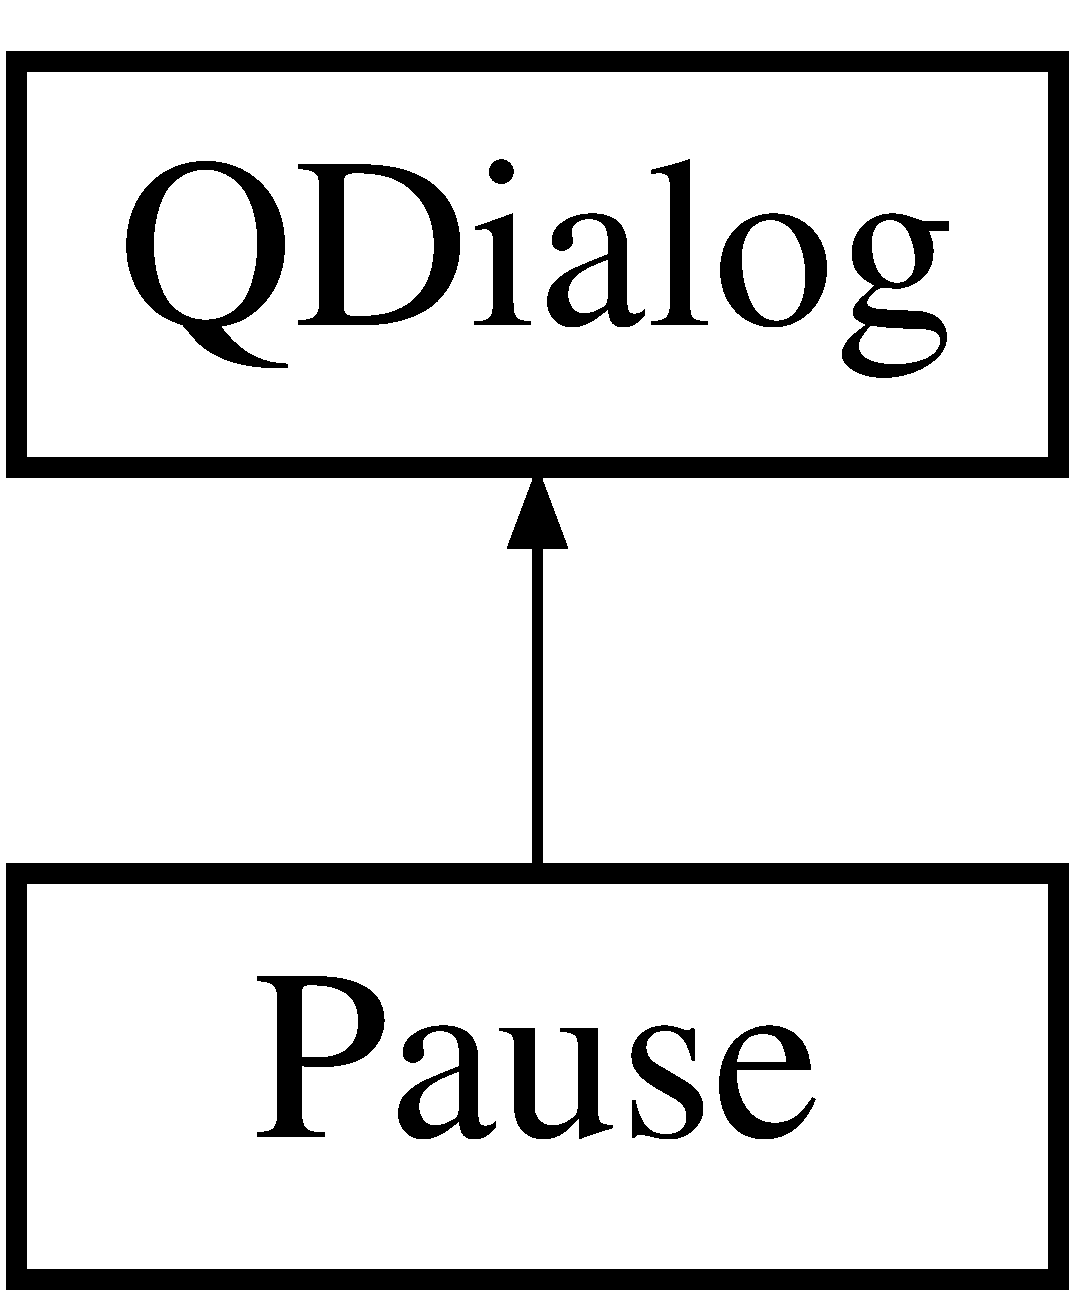
\includegraphics[height=2.000000cm]{class_pause}
\end{center}
\end{figure}
\subsection*{Public Slots}
\begin{DoxyCompactItemize}
\item 
\hypertarget{class_pause_ad632066c1f745b88f328f609de26419f}{void {\bfseries on\-\_\-resume\-\_\-clicked} ()}\label{class_pause_ad632066c1f745b88f328f609de26419f}

\item 
\hypertarget{class_pause_aed0cb80fa11b7556ffe285bb83696e55}{void {\bfseries on\-\_\-exit\-\_\-clicked} ()}\label{class_pause_aed0cb80fa11b7556ffe285bb83696e55}

\item 
\hypertarget{class_pause_a2b4c1e4ee50785bcca1dc1c422f527b3}{void {\bfseries on\-\_\-progress\-Bar\-\_\-value\-Changed} (int value)}\label{class_pause_a2b4c1e4ee50785bcca1dc1c422f527b3}

\end{DoxyCompactItemize}
\subsection*{Public Member Functions}
\begin{DoxyCompactItemize}
\item 
\hypertarget{class_pause_a2677e62030e9d138bc9994f9d6bd727b}{{\bfseries Pause} (Q\-Widget $\ast$parent=0)}\label{class_pause_a2677e62030e9d138bc9994f9d6bd727b}

\end{DoxyCompactItemize}
\subsection*{Public Attributes}
\begin{DoxyCompactItemize}
\item 
\hypertarget{class_pause_ac99bac0f2bea6e439f0d55ba32efe920}{\hyperlink{class_character}{Character} $\ast$ {\bfseries hero}}\label{class_pause_ac99bac0f2bea6e439f0d55ba32efe920}

\end{DoxyCompactItemize}


The documentation for this class was generated from the following files\-:\begin{DoxyCompactItemize}
\item 
pause.\-h\item 
pause.\-cpp\end{DoxyCompactItemize}

\hypertarget{classshotgun}{\section{shotgun Class Reference}
\label{classshotgun}\index{shotgun@{shotgun}}
}
Inheritance diagram for shotgun\-:\begin{figure}[H]
\begin{center}
\leavevmode
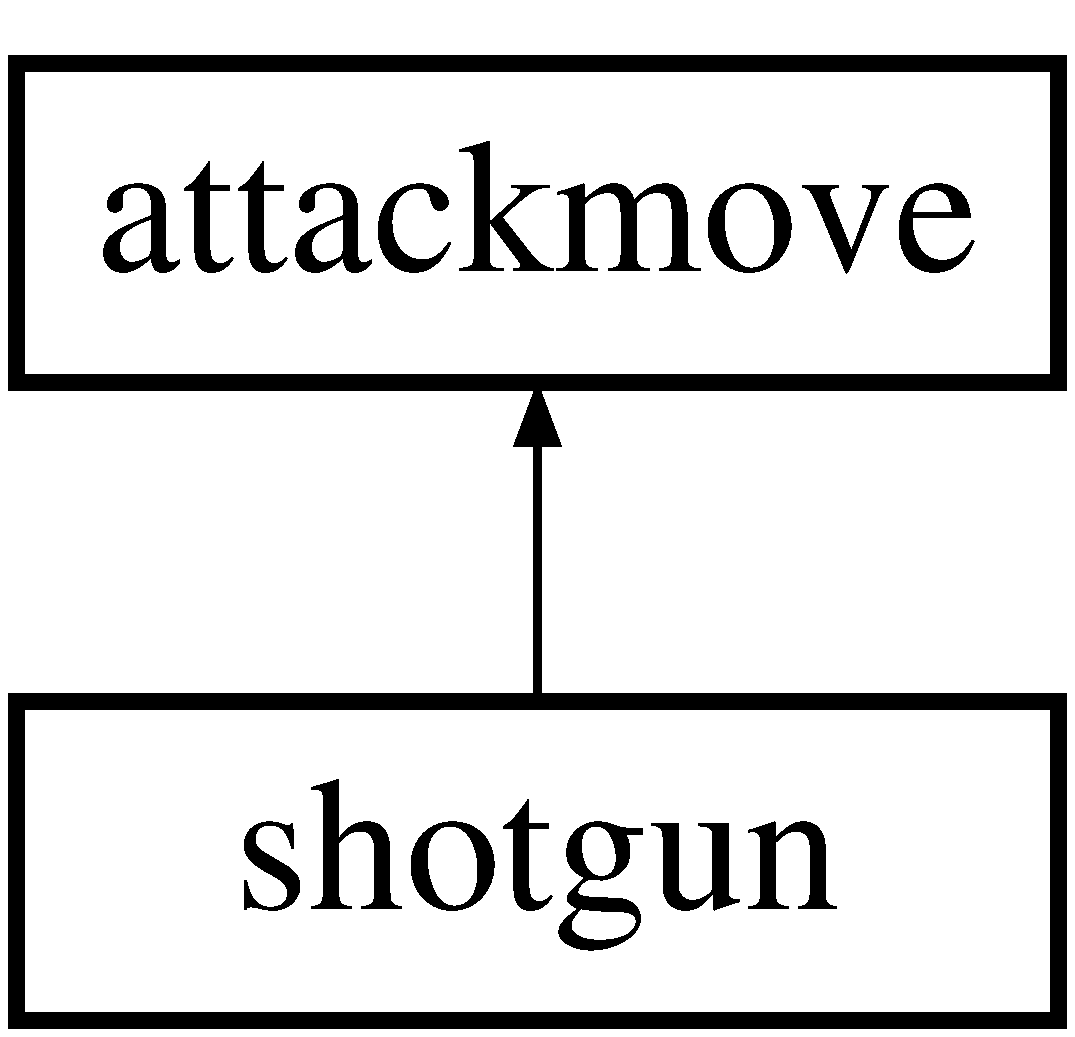
\includegraphics[height=2.000000cm]{classshotgun}
\end{center}
\end{figure}
\subsection*{Public Member Functions}
\begin{DoxyCompactItemize}
\item 
\hypertarget{classshotgun_adbc12267b0204869263cd2813fb6ccc1}{{\bfseries shotgun} (int dam)}\label{classshotgun_adbc12267b0204869263cd2813fb6ccc1}

\item 
\hypertarget{classshotgun_a856fa8335ee3c2bb8603e83aa5629e5c}{virtual Q\-String {\bfseries get\-String} ()}\label{classshotgun_a856fa8335ee3c2bb8603e83aa5629e5c}

\item 
\hypertarget{classshotgun_a1336af80f8d3f7d19ac954f2e616a1b0}{virtual Q\-Image {\bfseries get\-Image} ()}\label{classshotgun_a1336af80f8d3f7d19ac954f2e616a1b0}

\item 
\hypertarget{classshotgun_a8334202fd30d71432db7e58fca7a462e}{virtual void {\bfseries get\-Hover} (int hpanel, \hyperlink{class_enemy}{Enemy} $\ast$Enemies\mbox{[}3\mbox{]}, \hyperlink{classanim_items}{anim\-Items} $\ast$anim)}\label{classshotgun_a8334202fd30d71432db7e58fca7a462e}

\item 
\hypertarget{classshotgun_a38d2c751cb6f3bed896d8d71c5354de5}{virtual void {\bfseries do\-Attack} (int hpanel, \hyperlink{class_enemy}{Enemy} $\ast$Enemies\mbox{[}$\,$\mbox{]}, \hyperlink{classanim_items}{anim\-Items} $\ast$anim)}\label{classshotgun_a38d2c751cb6f3bed896d8d71c5354de5}

\end{DoxyCompactItemize}
\subsection*{Additional Inherited Members}


The documentation for this class was generated from the following files\-:\begin{DoxyCompactItemize}
\item 
shotgun.\-h\item 
shotgun.\-cpp\end{DoxyCompactItemize}

\hypertarget{class_skeleton}{\section{Skeleton Class Reference}
\label{class_skeleton}\index{Skeleton@{Skeleton}}
}
Inheritance diagram for Skeleton\-:\begin{figure}[H]
\begin{center}
\leavevmode
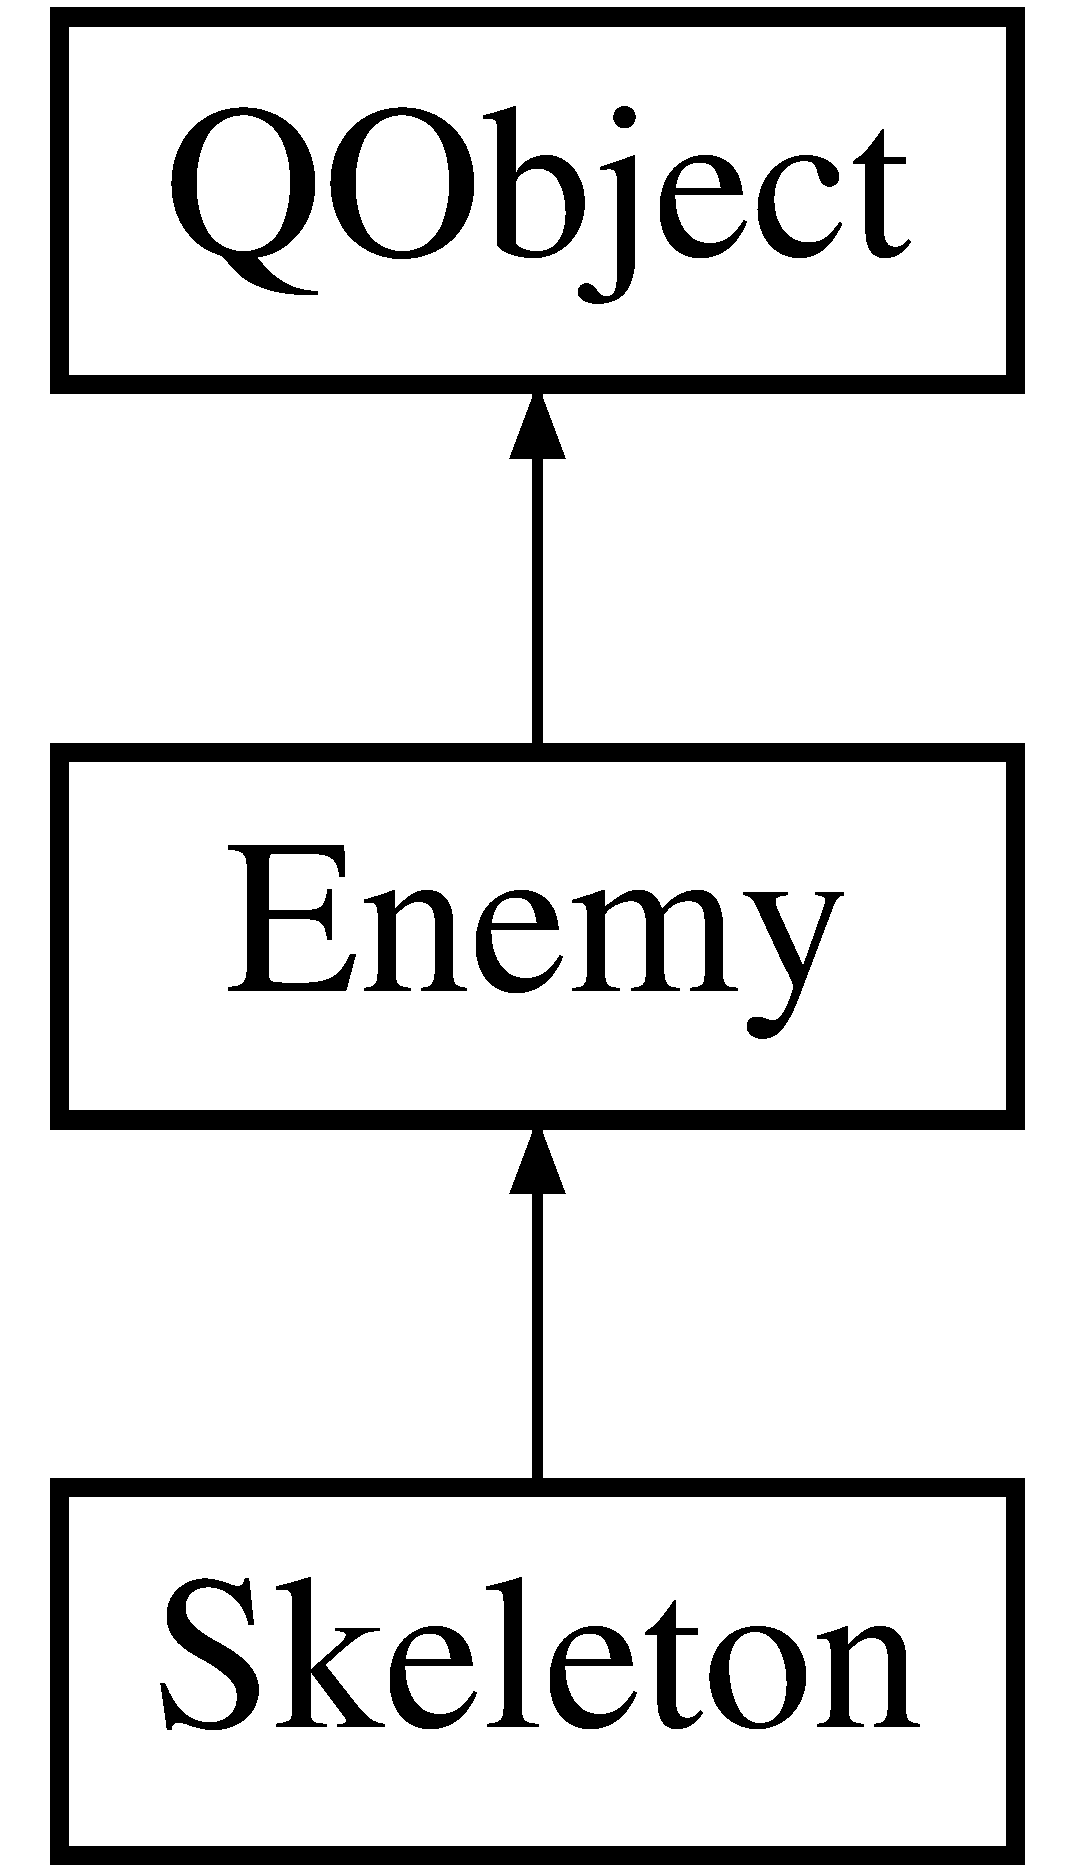
\includegraphics[height=3.000000cm]{class_skeleton}
\end{center}
\end{figure}
\subsection*{Public Member Functions}
\begin{DoxyCompactItemize}
\item 
\hypertarget{class_skeleton_ac4920b7ab446add4c8da5c8fe6aff2d3}{{\bfseries Skeleton} (int clev, int cx, int cy)}\label{class_skeleton_ac4920b7ab446add4c8da5c8fe6aff2d3}

\item 
\hypertarget{class_skeleton_aeb5642a3aa8c49cb0cd1cc325f8f0baa}{virtual void {\bfseries do\-Turn} (\hyperlink{class_character}{Character} $\ast$Hero)}\label{class_skeleton_aeb5642a3aa8c49cb0cd1cc325f8f0baa}

\item 
\hypertarget{class_skeleton_a35acfe2e2da4279a56d91bb8f2048489}{virtual Q\-Image {\bfseries get\-Pic} ()}\label{class_skeleton_a35acfe2e2da4279a56d91bb8f2048489}

\item 
\hypertarget{class_skeleton_ae605f24f6e921ad3b36a53f391304722}{virtual void {\bfseries draw\-Self} (Q\-Painter $\ast$g, int gx, int gy)}\label{class_skeleton_ae605f24f6e921ad3b36a53f391304722}

\end{DoxyCompactItemize}
\subsection*{Additional Inherited Members}


The documentation for this class was generated from the following files\-:\begin{DoxyCompactItemize}
\item 
skeleton.\-h\item 
skeleton.\-cpp\end{DoxyCompactItemize}

\hypertarget{classswordslash}{\section{swordslash Class Reference}
\label{classswordslash}\index{swordslash@{swordslash}}
}
Inheritance diagram for swordslash\-:\begin{figure}[H]
\begin{center}
\leavevmode
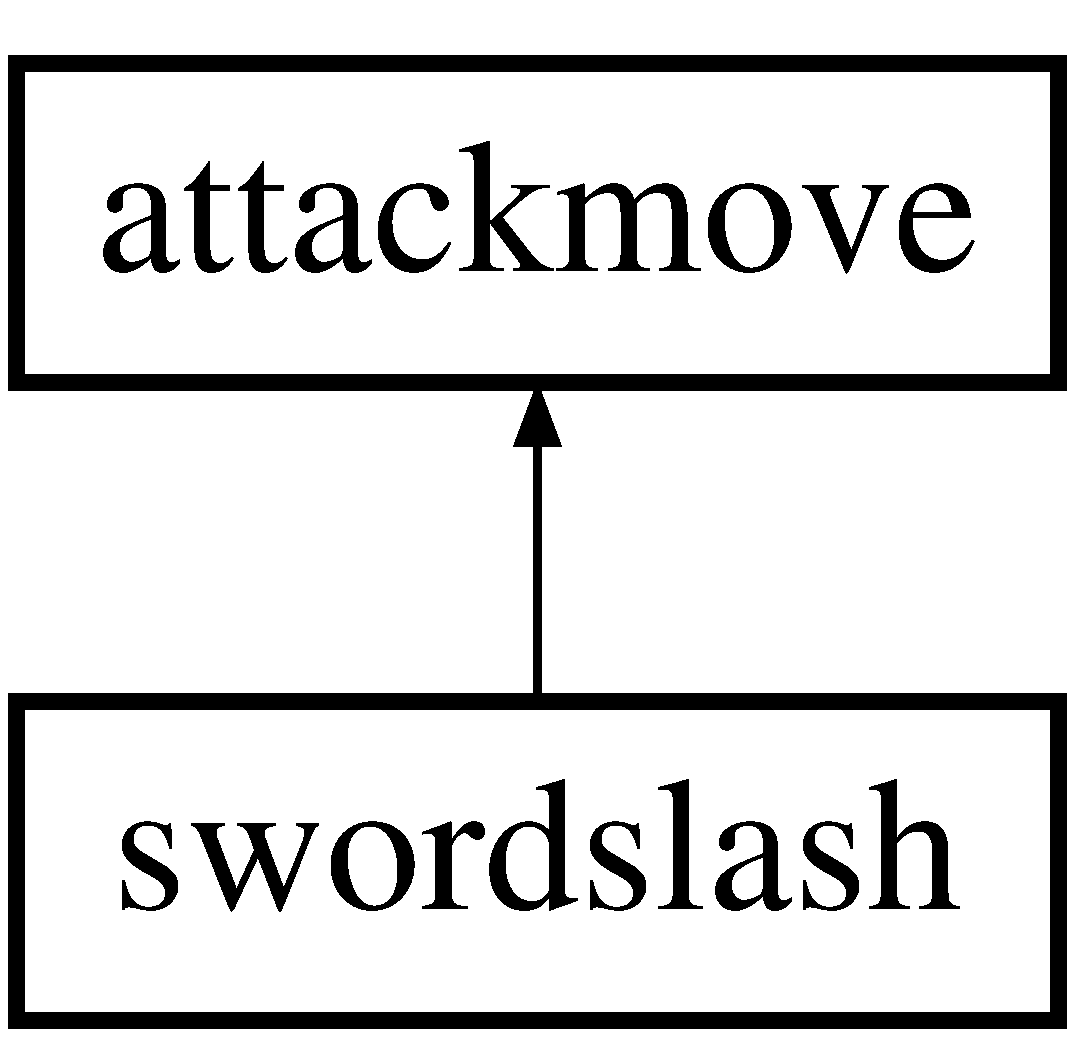
\includegraphics[height=2.000000cm]{classswordslash}
\end{center}
\end{figure}
\subsection*{Public Member Functions}
\begin{DoxyCompactItemize}
\item 
\hypertarget{classswordslash_a1c4547e783632e2e3e42642754dfb6ea}{{\bfseries swordslash} (int dam)}\label{classswordslash_a1c4547e783632e2e3e42642754dfb6ea}

\item 
\hypertarget{classswordslash_ac58a7e3b969bb957548c55bdfd6a0b05}{virtual Q\-String {\bfseries get\-String} ()}\label{classswordslash_ac58a7e3b969bb957548c55bdfd6a0b05}

\item 
\hypertarget{classswordslash_a25cbfa2df6b5718a299eed09cf716822}{virtual Q\-Image {\bfseries get\-Image} ()}\label{classswordslash_a25cbfa2df6b5718a299eed09cf716822}

\item 
\hypertarget{classswordslash_af40c617c0463f788bda02fe5e8109511}{virtual void {\bfseries get\-Hover} (int hpanel, \hyperlink{class_enemy}{Enemy} $\ast$Enemies\mbox{[}3\mbox{]}, \hyperlink{classanim_items}{anim\-Items} $\ast$anim)}\label{classswordslash_af40c617c0463f788bda02fe5e8109511}

\item 
\hypertarget{classswordslash_a8583edccf2f8b5635797e6891f797211}{virtual void {\bfseries do\-Attack} (int hpanel, \hyperlink{class_enemy}{Enemy} $\ast$Enemies\mbox{[}$\,$\mbox{]}, \hyperlink{classanim_items}{anim\-Items} $\ast$anim)}\label{classswordslash_a8583edccf2f8b5635797e6891f797211}

\end{DoxyCompactItemize}
\subsection*{Additional Inherited Members}


The documentation for this class was generated from the following files\-:\begin{DoxyCompactItemize}
\item 
swordslash.\-h\item 
swordslash.\-cpp\end{DoxyCompactItemize}

\hypertarget{classswordsman}{\section{swordsman Class Reference}
\label{classswordsman}\index{swordsman@{swordsman}}
}
Inheritance diagram for swordsman\-:\begin{figure}[H]
\begin{center}
\leavevmode
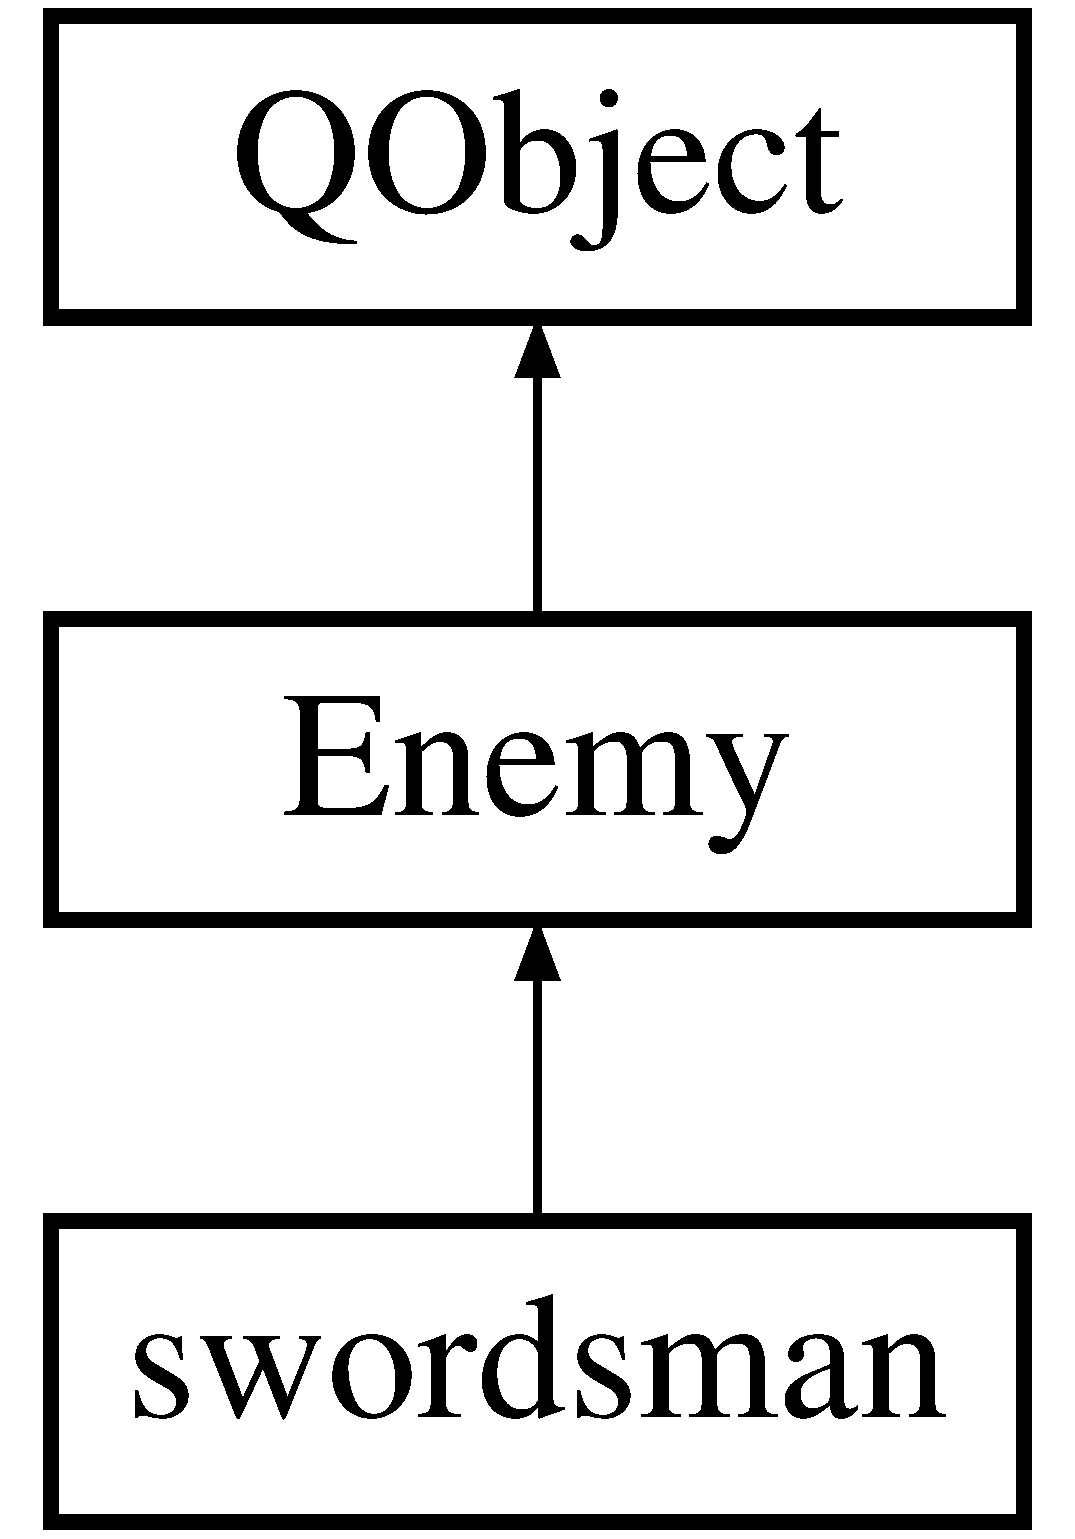
\includegraphics[height=3.000000cm]{classswordsman}
\end{center}
\end{figure}
\subsection*{Public Member Functions}
\begin{DoxyCompactItemize}
\item 
\hypertarget{classswordsman_afa4407146d49326932f9b1fa4f97ab2d}{{\bfseries swordsman} (int clev, int cx, int cy)}\label{classswordsman_afa4407146d49326932f9b1fa4f97ab2d}

\item 
\hypertarget{classswordsman_a99dec33c47dc5f3936229e5045b9c235}{virtual void {\bfseries do\-Turn} (\hyperlink{class_character}{Character} $\ast$Hero)}\label{classswordsman_a99dec33c47dc5f3936229e5045b9c235}

\item 
\hypertarget{classswordsman_a68098988c90a499ebfb757c7750bae7f}{virtual Q\-Image {\bfseries get\-Pic} ()}\label{classswordsman_a68098988c90a499ebfb757c7750bae7f}

\item 
\hypertarget{classswordsman_ad897e7c34033347faa5e4022b27cc395}{virtual void {\bfseries draw\-Self} (Q\-Painter $\ast$g, int gx, int gy)}\label{classswordsman_ad897e7c34033347faa5e4022b27cc395}

\end{DoxyCompactItemize}
\subsection*{Additional Inherited Members}


The documentation for this class was generated from the following files\-:\begin{DoxyCompactItemize}
\item 
swordsman.\-h\item 
swordsman.\-cpp\end{DoxyCompactItemize}

\hypertarget{classworldmap}{\section{worldmap Class Reference}
\label{classworldmap}\index{worldmap@{worldmap}}
}
Inheritance diagram for worldmap\-:\begin{figure}[H]
\begin{center}
\leavevmode
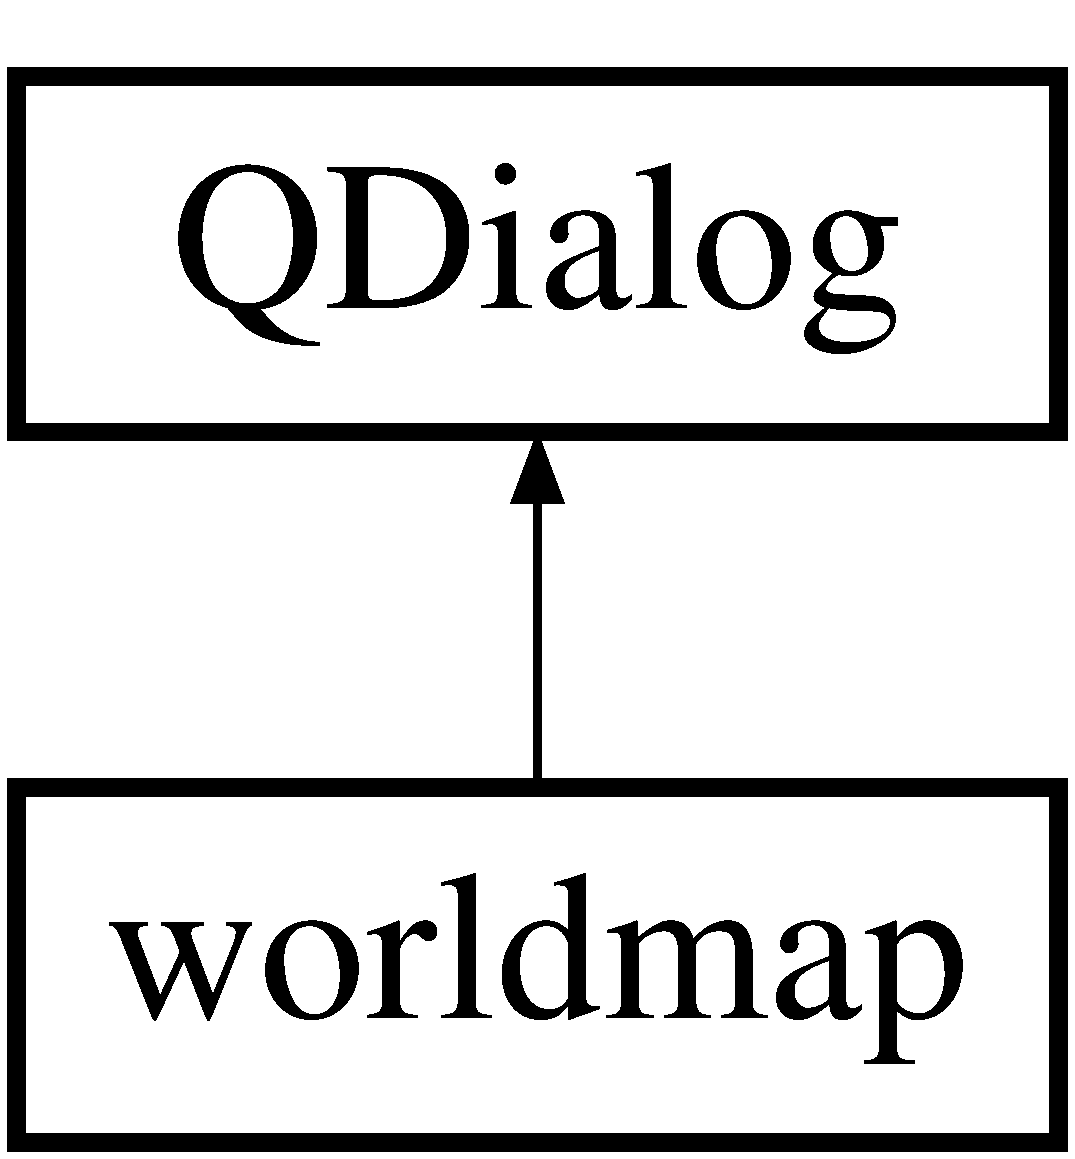
\includegraphics[height=2.000000cm]{classworldmap}
\end{center}
\end{figure}
\subsection*{Public Member Functions}
\begin{DoxyCompactItemize}
\item 
\hypertarget{classworldmap_a970f51f58c07cc43b110fecf43519838}{{\bfseries worldmap} (Q\-Widget $\ast$parent=0)}\label{classworldmap_a970f51f58c07cc43b110fecf43519838}

\end{DoxyCompactItemize}


The documentation for this class was generated from the following files\-:\begin{DoxyCompactItemize}
\item 
worldmap.\-h\item 
worldmap.\-cpp\end{DoxyCompactItemize}

\hypertarget{classxgun}{\section{xgun Class Reference}
\label{classxgun}\index{xgun@{xgun}}
}
Inheritance diagram for xgun\-:\begin{figure}[H]
\begin{center}
\leavevmode
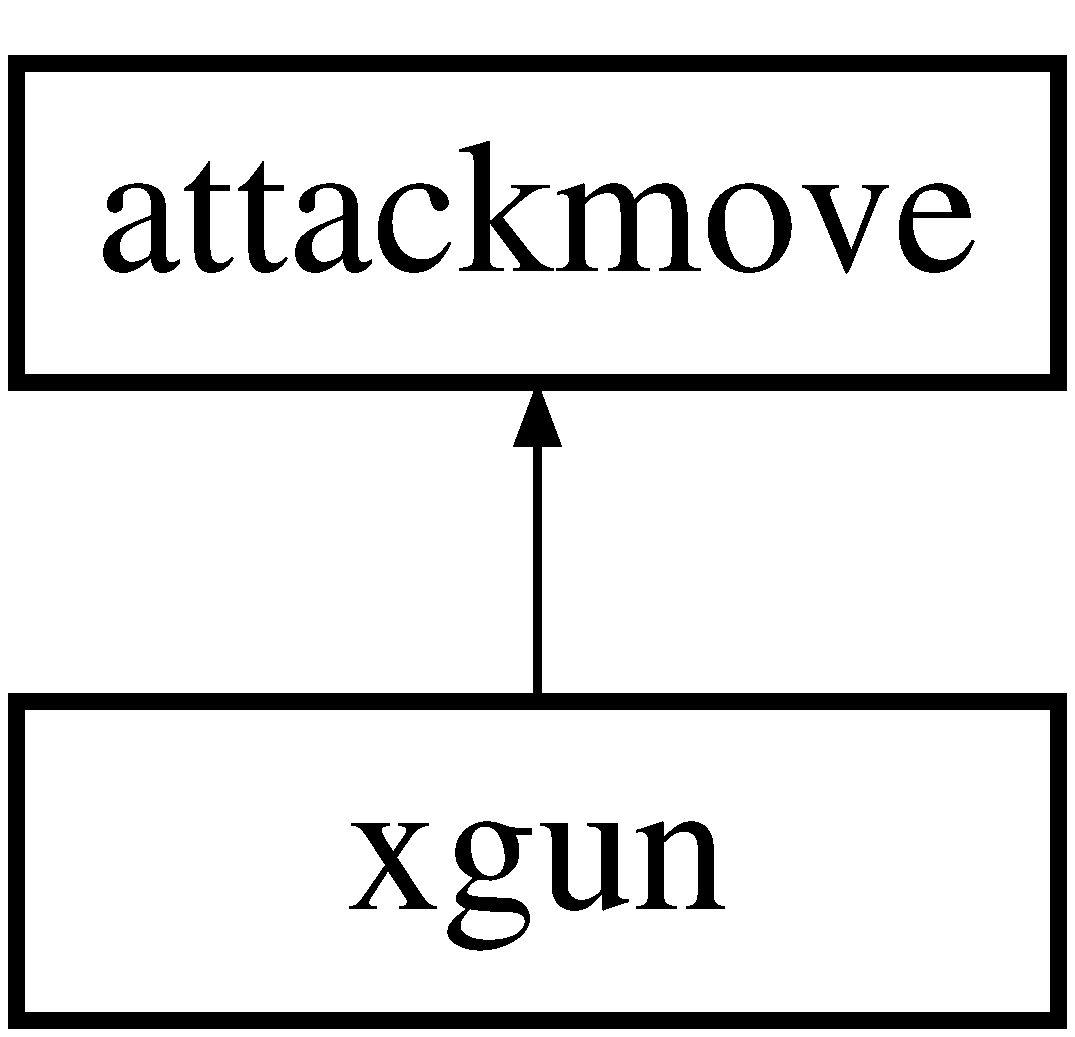
\includegraphics[height=2.000000cm]{classxgun}
\end{center}
\end{figure}
\subsection*{Public Member Functions}
\begin{DoxyCompactItemize}
\item 
\hypertarget{classxgun_a559665713dc1ae233184807d8b38ab7f}{{\bfseries xgun} (int dam)}\label{classxgun_a559665713dc1ae233184807d8b38ab7f}

\item 
\hypertarget{classxgun_a8d091859d655ff1703630ba7dd88a358}{virtual Q\-String {\bfseries get\-String} ()}\label{classxgun_a8d091859d655ff1703630ba7dd88a358}

\item 
\hypertarget{classxgun_adf5511bd6ed5dfb184a8a3b6b757608a}{virtual Q\-Image {\bfseries get\-Image} ()}\label{classxgun_adf5511bd6ed5dfb184a8a3b6b757608a}

\item 
\hypertarget{classxgun_aac799bda61860430dbbd9403b80a1efd}{virtual void {\bfseries get\-Hover} (int hpanel, \hyperlink{class_enemy}{Enemy} $\ast$Enemies\mbox{[}$\,$\mbox{]}, \hyperlink{classanim_items}{anim\-Items} $\ast$anim)}\label{classxgun_aac799bda61860430dbbd9403b80a1efd}

\item 
\hypertarget{classxgun_a8ede91a770bcedc6c4454615d38b5e84}{virtual void {\bfseries do\-Attack} (int hpanel, \hyperlink{class_enemy}{Enemy} $\ast$Enemies\mbox{[}$\,$\mbox{]}, \hyperlink{classanim_items}{anim\-Items} $\ast$anim)}\label{classxgun_a8ede91a770bcedc6c4454615d38b5e84}

\end{DoxyCompactItemize}
\subsection*{Additional Inherited Members}


The documentation for this class was generated from the following files\-:\begin{DoxyCompactItemize}
\item 
xgun.\-h\item 
xgun.\-cpp\end{DoxyCompactItemize}

%--- End generated contents ---

% Index
\newpage
\phantomsection
\addcontentsline{toc}{part}{Index}
\printindex

\end{document}
